\documentclass[10pt,conference]{IEEEtran}
\IEEEoverridecommandlockouts
% The preceding line is only needed to identify funding in the first footnote. If that is unneeded, please comment it out.
\usepackage{cite}
\usepackage{amsmath,amssymb,amsfonts}
%\usepackage{algorithmic}
\usepackage{graphicx}
\usepackage{textcomp}
\usepackage{xcolor}
\usepackage{tikz}
\usepackage{multirow}
\usetikzlibrary{arrows.meta}
\usepackage{subcaption}
\usepackage{todonotes}
\usepackage{multirow}
\usepackage{xspace}
\usepackage{hyperref}
\usepackage{url}
\usepackage{comment}

\def\BibTeX{{\rm B\kern-.05em{\sc i\kern-.025em b}\kern-.08em
    T\kern-.1667em\lower.7ex\hbox{E}\kern-.125emX}}
\begin{document}

\newcommand\schim{SchIM\xspace}
\newcommand\schimL{Scheduler In-the-Middle\xspace}
\newcommand\schiml{scheduler in-the-middle\xspace}
\newcommand\axiin[1]{$\texttt{HPM}_{#1}$\xspace}
\newcommand\axiout[1]{$\texttt{HPS}_{#1}$\xspace}
\newcommand\axiconf[1]{$\texttt{LPM}_{#1}$\xspace}

\newcommand{\fig}[1]{Fig.~\ref{#1}}

\newcommand*\circledfig[2]{Fig.~\ref{#1}\tikz[baseline=0pt]{\node[anchor=south west,red,shape=circle,draw,inner sep=1pt] (char) {\scriptsize#2};}}

\newcommand*\circled[1]{\tikz[baseline=0pt]{\node[anchor=south west,red,shape=circle,draw,inner sep=1pt] (char) {\scriptsize#1};}}

\title{A Memory Scheduling Infrastructure for Multi-core Systems with
  Re-programmable Logic
%    \thanks{Identify applicable funding agency here. If none, delete this.}
}

\author{
%    \IEEEauthorblockN{1\textsuperscript{st} Given Name Surname}
%    \IEEEauthorblockA{
%        \textit{dept. name of organization (of Aff.)} \\
%        \textit{name of organization (of Aff.)}\\
%        City, Country \\
%        email address or ORCID
%    }
%    \and
%    \IEEEauthorblockN{2\textsuperscript{nd} Given Name Surname}
%    \IEEEauthorblockA{
%        \textit{dept. name of organization (of Aff.)} \\
%        \textit{name of organization (of Aff.)}\\
%        City, Country \\
%        email address or ORCID
%    }
%    \and
%    \IEEEauthorblockN{3\textsuperscript{rd} Given Name Surname}
%    \IEEEauthorblockA{
%        \textit{dept. name of organization (of Aff.)} \\
%        \textit{name of organization (of Aff.)}\\
%        City, Country \\
%        email address or ORCID
%    }
    Authors omitted for review.
}

\maketitle

\begin{abstract}
  TBD
\end{abstract}

\begin{IEEEkeywords}
component, formatting, style, styling, insert
\end{IEEEkeywords}

\section{Introduction}
    In modern embedded Mutli-core Systems, caches have become an angular piece of hardware bridging the gap between the speed of the connected execution units and the main memory. With the growing demand for high-performance multi-core system on chips, shared caches have evolved to accomodate the many concurrent accesses to main memory and increase the cache hit-rate. These caches are referred to as \emph{non-blocking}.\\

    Unfortunately, while non-blocking shared caches offer great average perfomance, their behaviour is opaque and unpredictable. Dealing with the cache behaviour is of the utmost importance for safety critical hard Real-Time systems where timing constraints must be respected and guaranteed. A great deal of research has been conducted on cache management for Real-Time applications on MPSoCs. The two main sources of unpredictability imputed to the last-level of cache are (1) the inter-core cache line eviction and (2) the opaque management of internaly shared resources.

    The inter-core cache line eviction is a well studied source of unpredictability that arises when the memory accesses of two independent cores lead to the eviction of each others cache line in a destructive way. Such source of unpredictability can be addressed and mitigated by enforcing the \emph{spacial isolation} of the cores. Both software solutions (e.g. via cache coloring \cite{}) and hardware solutions (e.g. via lockdown per master \cite{Giovani_cahe_partitioning_survey}) are available and commonly used.

    Inter-core interferences caused by internal shared resources such as the \emph{Miss-Status-Holding-Registers} (MSHR) or the \emph{write-back} unit  have been recently studied. In \cite{Valsan2017AddressingIC, Heechul_DDOS_attacks_on_shared_cache}, the authors have shown that these shared resources can introduce a consequent amount of interference, mutiply the exeuction time of the tasks running on the victim core by a factor of 346. Such conditions only occur when the attacker creates extrem contention in the write-back unit, resulting in a head-of-the-line-blocking.\\

    In the present article, we show that on the ARM Cortex-A53 \cite{ARM-cortex-A53} a third source of inter-core interferences exists: the target memory response time. In addition, we demonstrate that, in contrary to what has been shown before, read transactions can also caused interferrences. More accurately, we show that if a target memory ackownledges the transaction, but waits to deliver the response, the execution time of tasks running on independent cores can be impacted by a factor of 11. Furthermore, we show that if this single read transaction is acknowledged by the target memory, but the latter never provides a response, the whole core cluster is frozen indefinitely. To the best of our knowledge, this is the first report demonstrating that a core cluster can be subject to interferences caused by a single isolated read transaction.\\

    The present article is organised as follows: TODO

\section{Related work}
    An important amount of research has focused on addressing the challenges of isolating the cores sharing the same cache and thus, preventing unpredictable behaviour such as increased in execution time.
    Most of this research \cite{Mancuso2013RealtimeCM, 6755286} has aimed at \emph{spacially isolating} the cores (i.e. avoiding inter-core cache line eviction by constraining each core data and instructions in a specific region of the shared cache). Hardware based solutions such as \emph{lockdown per way} \cite{Giovani_cahe_partitioning_survey} are efficient, but not integrated in every platforms.
    On the other hand, software based solutions such as cache coloring \cite{Mancuso2013RealtimeCM} can be deployed in most platforms, but comes at the cost of increased memory space requirements.

    However, recent research \cite{Valsan2017AddressingIC, Heechul_DDOS_attacks_on_shared_cache} have highlighted that, while cache partitioning is successful in most cases, in some situations, contention on shared internal units such as the MSHRs or the write-back unit can also introduce substential inter-core interferences.
    In \cite{Valsan2017AddressingIC}, the authors evaluate the impact of inter-core interference originated by the MSHRs on multiple platforms and propose a solution to eliminate this contention. The solution is based on a combination of a small hardware module and an OS-level controller.
    Their experiments show that, if let unmanaged, the execution time of independent cores is multiplied by 10.6 and 21.3 under read and write workloads, respectively.
    By the mean of simulation, they prove that their approach is successful at providing the best overall throughput for each core while suppressing the inter-core interference caused by the MSHRs.
    % Running applicative benchmarks, increas in execution time of a factor of 6.4 have been observed.
    \cite{Heechul_DDOS_attacks_on_shared_cache} investigates the contention in caches caused by shared internal units in the case of \emph{Denial-of-service} (DOS) attacks and propose an OS-level solution enabling finer management of the system bandwidth.
    In contrast to \cite{Valsan2017AddressingIC}, the internal unit studied and exploited is the write-back unit.
    They report that, by exploiting this unit efficiently, one can increase the execution time of a victim task by a factor of 346.

\section{System Background}
\subsection{Cache and DRAM temporal partitioning}

\subsection{Programmable Logic in the Middle(PLIM)}

Here we detail the necessary background to understand how to interpose a module between a traditional multi-core processor and main memory.

Commercially available SoCs that integrate a traditional embedded multi-core processor system (PS) and a block of programmable logic (PL) with high-performance PS-PL communication interfaces. There are high-performance masters (HPM) and high-performance slaves (HPS) to send and receive transactions to and from the PL, respectively.

The underlying mechanism is the ability to intercept memory transactions originated from the processors inside the PS, at the PL. Transactions are then forwarded from the PL again toward the memory controller inside the PS. The primary mechanism of PS-PL and PL-PS redirection of a transaction is called the Memory Loop-Back. Loop-Back is done through address bit manipulation of the transaction such that it falls in the range of the target HPM(HPS) for the PS-PL(PL-PS) interception. In this way, the main memory content is accessed, but through a programmable environment. It is possible to act on the characteristics of the traffic that now traverses the PL. For example, in the PL, it is possible to direct the transaction to arbitrary modules before, eventually, redirecting it back to PS and the memory controller, ultimately.

This provides a unique capability of manipulating individual memory transactions. Hence, by sitting between CPUs and main memory, PLIM is exploited to perform memory scheduling. A configurable memory scheduler in the middle, namely SchIM, is designed to implement several elected scheduling policies of Fixed Priority, TDMA, and Memguard. With
SchIM, now we can enforce policy at the level of the transaction altogether by the hardware.



\subsubsection{PS-PL SoCs}
\subsubsection{Advanced eXtensible Interface (AXI)}
\subsubsection{Memory-Loopback}
\subsubsection{Cache Bleaching}
\subsubsection{Transaction-level Inspection}
\subsubsection{Transaction-level Profiling}

\subsection{Jailhouse, the partitioning Hypervisor}
\subsubsection{Partitioning}
        \subsubsection{Run-time Zero-Copy Recoloring support}

\section{Design Goals and Overview}\label{sec:overview}

%% General introduction about the SchIM
In this section, we introduce the proposed \schim design and describe
the overarching goals of this work. We then provide a bird's-eye view
of the \schim organization and principles of operation.

\subsection{Design Goals}\label{sec:design_goals}
As briefly surveyed in Section~\ref{sec:relwork}, there have been
numerous proposals for better memory controllers and approaches to
manage memory traffic in modern multi-core embedded platforms. With
respect to the existing literature, the purpose of this work is
twofold. First, we want to demonstrate that scheduling CPU-originated
memory traffic at the granularity of individual transactions is
possible in PS-PL platforms. Second, and more importantly, we want to
provide an infrastructure that is generic and extensible enough for
the broader research community to adopt and foster a new chapter on
PL-assisted memory scheduling. With this in mind, we establish the
following goals.

\par{\bf Extensible memory scheduling infrastructure.} First and
foremost, the \schim has been designed with modularity and
extensibility in mind. We separate the functionalities that concern
handling, queuing, selection, and forwarding of memory requests inside
our infrastructure. Moreover, we design our \schim to be able to
simultaneously support multiple memory scheduling policies. A simple,
standardized interface is provided to define new memory scheduling
policies without impacting the design of the rest of the \schim. We
discuss in Section~\ref{sec:sched_interf} the generic interface
provided by the \schim to implement a new memory scheduling policy.

\par{\bf Runtime configuration and transparency.} We want the \schim
to be a powerful supporting infrastructure to evaluate, compare, and
contrast memory scheduling policies. As such, we strive to provide (1)
runtime reconfigurability and (2) operational transparency. By
allowing memory scheduling policies to be switched at runtime, it is
possible to rapidly identify desirable configuration parameters or to
tune the adopted scheduling policy to workload criticality and memory
intensiveness. For this purpose, the \schim exposes a memory-mapped
configuration interface where all the operational parameters can be
changed at runtime. At the same time, we want to ensure that the
applications and the (real-time) operating system under analysis need
not to be modified to use the \schim. Hence, we propose the use of a
thin virtualization layer to selectively route memory traffic through
the \schim without changes to the binary of OS kernel and
applications.

\par{\bf Realistic performance with experimental policies.} One of the
limiting factors of research on memory scheduling policies is the
ability to construct evidence of performance improvements with
realistic workload. Proposing a new memory scheduling policy is
traditionally done with either a simulated setup, or with a
full-system soft-core implementation. In both cases, the timescale of
experiment collection is orders of magnitude slower than what it would
be in a real systems. This forces the use of unrealistically
lightweight workload and limits the repeatability of experiments of
scale. Furthermore, the multi-fold drop in performance excludes the
possibility of adopting experimental memory scheduling policies for a
production-ready system. Conversely, we envision that our \schim will
be an intermediate step in the transition path to production of
research-seeded ideas. Additionally, as PS-PL platforms mature and the
interplay of PL and memory resources improves, a \schim-like design
could be the way to go for mission-reconfigurable, upgradable embedded
systems.

\subsection{Design Overview}
As previously mentioned, the \schim leverages the PLIM
approach. CPU-originated main memory transactions are re-routed
through the programmable logic and scheduled by the \schim according
to a flexible and configurable policy. The result is that the timing
of memory transactions generated by real-time applications can be
carefully determined and reasoned upon. Because the \schim follows a
PLIM approach, transactions can be selectively sent to the \schim for
scheduling. It is always possible, however, to dynamically exclude the
\schim and instead route transactions directly to main memory. For the
purpose of this paper we consider a setup in which all the
CPU-generated memory transactions are handled by the \schim.

%% First and foremost, SchIM follows a selective and dynamic re-routing
%% policy settled at the run-time, meaning that provided a proper routing
%% configuration interface, SchIM can be bypassed if unacceptable
%% overhead for some applications is detected by going through the PL
%% following the Loop-Back routing strategy. Additionally, SchIM,
%% provides a safe production-ready environment on COTS platforms where
%% one can enfroce and test any proposed scheduling policy at the level
%% of the transaction altogether by the real hardware. Memory scheduling
%% traditionally done via hardware modifications at the controller level,
%% or solely via software. Providing SchIM, we are now able to transcend
%% this on intact COTS to conduct an analysis of feasibility, challenges
%% and performance.

Figure~\ref{fig:block_diagram} provides an overview of the location of
the \schim within the main components of the target platform. The
highlighted {\bf COLOR} path depicts the route that memory requests
originated by the CPUs follow when the SchIM is used. Application
memory requests can reach the \schim through multiple
interfaces. Without loss of generality, we consider a \schim instance
with two arrival lanes, which are labeled as \axiin{1} and \axiin{2}
in Figure~\ref{fig:block_diagram}. The \schim then forwards the
received transactions towards main memory through the \axiout{3}
interface. A more detailed view of the \schim module is provided in
Figure~\ref{fig:MemorEDF_module_schema} where the same convention is
used to identify input and output ports. In addition, as shown in
Figure~\ref{fig:MemorEDF_module_schema}, a fourth \axiconf{4} port is
used to configure the \schim module from the PS.

%% The objective of the module is to arbitrate the access of the bus to
%% the main memory between the different cores of the PS side at the
%% transaction level by enforcing a given policy.  Roughly, the module
%% receives transactions from the PS side, acknowledges them and finally
%% repeat them with the main memory as destination.  The exact order in
%% which inter-core transactions are being repeated is decided by an
%% embedded on-chip hardware scheduler.

%% \begin{figure}
%%   \centering
%%   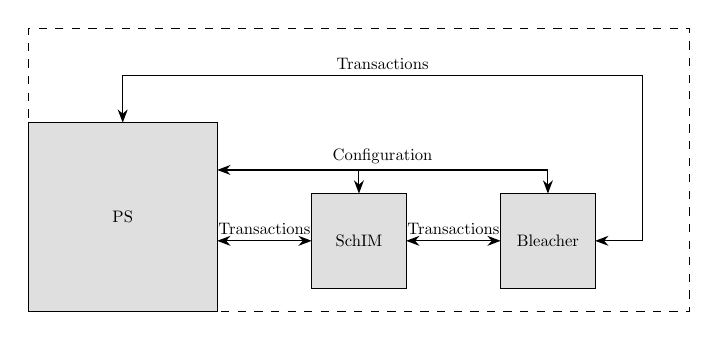
\begin{tikzpicture}[scale=0.6, every node/.style={scale=0.6}]
    % Modules
    \draw[fill={rgb:black,1;white,7}] ( 0.0, 0.0) rectangle ( 4.0, 4.0) node[pos=.5] {PS};
    \draw[fill={rgb:black,1;white,7}] ( 6.0, 0.5) rectangle ( 8.0, 2.5) node[pos=.5] {SchIM};
    \draw[fill={rgb:black,1;white,7}] (10.0, 0.5) rectangle (12.0, 2.5) node[pos=.5] {Bleacher};
    % Outline PL
    \draw[dashed] ( 0.0, 4.0) -- ( 4.0, 4.0) -- ( 4.0, 0.0) -- (14.0, 0.0) -- (14.0, 6.0) -- ( 0.0, 6.0) -- ( 0.0, 4.0);
    % Buses
    % PS to SchIM HPM0
    \draw[{Stealth}-{Stealth}] ( 4.0, 1.5) -- ( 6.0, 1.5) node[above, pos=.5] {Transactions};
    % SchIM to Bleacher HPM0
    \draw[{Stealth}-{Stealth}] ( 8.0, 1.5) -- (10.0, 1.5) node[above, pos=.5] {Transactions};
    % SchIM to Bleacher HPM0
    \draw[{Stealth}-{Stealth}] (12.0, 1.5) -- (13.0, 1.5) -- (13.0, 5.0) -- ( 2.0, 5.0) node[above, pos=.5] {Transactions} -- ( 2.0, 4.0);
    % PS to SchIM and Bleacher LPD
    \draw[{Stealth}-{Stealth}] ( 4.0, 3.0) -- (11.0, 3.0) node[above, pos=.5] {Configuration} -- (11.0, 2.5);
    \draw[-{Stealth}] ( 7.0, 3.0) -- ( 7.0, 2.5);
\end{tikzpicture}

%%   \caption{High-level block design of the proposed \schim
%%     module. \emph{RM: we need to replace this picture with one that
%%       provides more details about the main blocks of the platforms. We
%%       also do not need to include the bleacher as it is not
%%       fundamental for the operation of the \schim.}}
%%   \label{fig:SchIM_overview_schema}
%% \end{figure}


%% Micro-architecture and first list of modules
The \schim module is composed of a number of sub-modules grouped into
three different domains, namely (i) the \emph{interfacing domain},
(ii) the \emph{queuing domain}, and (iii) the \emph{scheduling
  domain}.

\par{\bf The interfacing domain} encompasses the sub-modules in charge
of interfacing the core logic of the \schim with the rest of the
system using the AXI protocol.  This domain is comprised of three
sub-modules. These are (i) the \emph{packetizer}, (ii) the
\emph{serializer}, and (iii) the previously mentioned configuration
interface.

The PS-facing end of the {\bf packetizer} offers an AXI slave port to
accept new incoming transactions. Upon receipt, this module transforms
each transaction into an equivalent \emph{packet} that can be queued
and scheduled by the rest of the \schim. Packetization of AXI
transactions is necessary to be able to store transactions that are
serial by nature.  Indeed, a standard AXI transaction is composed of
one address phase (AR or AW channel) followed by a data phase (R or W
channel) which can be itself composed of multiple successive bursts.

In many ways, the {\bf serializer} is the dual module of the
packetizer. Its purpose is to transform the packets that encode
CPU-generated memory requests back into AXI-compliant transactions. As
such, the serializer offers a master port to the rest of the system to
be routed to the main memory controller.

%% purpose of slave and master ports, they are also in charge of
%% respectively transforming the AXI transactions into an equivalent
%% packet and to transform these packets 

\par{\bf The queuing domain} handles how packets are stored between
receipt and re-trasnmission. This domain is comprised of (i) the
dispatcher module, (ii) the transaction queues, and (iii) the selector
module.

The use of {\bf multiple transaction queues} is necessary to
differentiate the traffic of the CPU cores and perform scheduling. As
such, the \schim associates a queue to each of the active cores ---
four in the platform of reference.
%% Therefore, in order to cancel the Round Robin arbitration policy
%% applied in the PS side and in order to avoid that one high priority
%% core is stalled by a lower priority one, each core is granted a queue
%% within the \schim module. <-- This should be obvious (RM)
The queues implemented in the \schim not only act as a holding space
for in-flight memory transactions.  They also (a) provide information
to the scheduling domain regarding their current state, and (b) they
can generate a congestion control signal to the associated CPU core.

As suggested by figure \ref{fig:MemorEDF_module_schema}, transactions
are categorized and enqueued based on the source of traffic. The {\bf
  dispatcher} module performs the matching between an incoming
transaction and the destination queue. Similarly, transactions are
dequeued by the {\bf selector} module and sent directly to the output
of the \schim following the decisions of the scheduling
domain.

\todo[inline]{RM:Briefly mention about the head-of-line blocking and
  regulation mechanism} Additional important details about the
categorization and congestion control mechanisms enacted in the
queueing domain are provided in
Section~\ref{sec:schim_implementation}.

\begin{figure*}
  \centering
  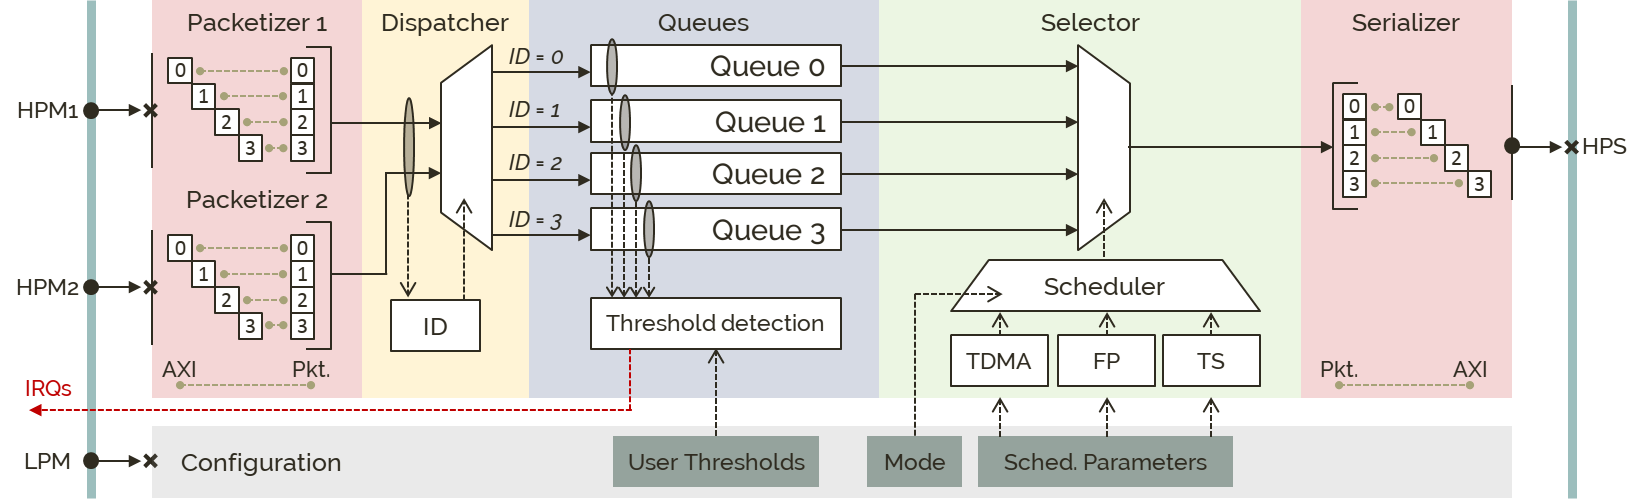
\includegraphics[width=0.8\textwidth]{images/SchIM_diagram.png}
  \caption{Caption}
  \label{fig:MemorEDF_module_schema}
\end{figure*}

\par{\bf The scheduling domain} encompasses all the sub-modules that
enable arbitration of transactions issued by the different cores of
the PS. The modules in this domain are intended to be generic for
extensibility, albeit a first set of three template schedulers is
provided as a proof of concept.  The scheduling policies currently
implemented in the \schim are Fixed Priority (FP), Time Division
Multiple Access (TDMA), and Budget-based Traffic Shaping (TS).  Each
of the parameters required by the implemented policies --- such as the
priorities, the periods, and the budgets --- can be adjusted at
run-time via the configuration interface.

The FP scheduler allows associating a priority value to each of the
transaction queues. Pending transactions at the queues are then
forwarded out of the \schim following the user-defined priority
order. The TDMA scheduler allows associating a transmission time slot
to each of the queues expressed in PL clock cycles. The module then
builds a schedule by concatenating the per-core slots so that only
pending transactions from one queue at a time are forwarded by the
\schim. Finally, with the TS scheduler, it is possible to associate a
maximum rate at which transactions from each queue are forwarded by
the \schim. 

%% Finally, the scheduling domain is also the one in charge of the
%% control of the remaining \schim module, driving and selecting the
%% adequate signals and ensuring the coherence and integrity of the data.

%% \subsection{Modules Overview}

%% \par{\bf Packetizer:} The packetizer module transforms transactions on
%% the asynchronous AXI bus into schedulable entities to be queued at any
%% of the \schim queues.


%\section{Theoretical Background}
    \subsection{Fixed Priority}
    \subsection{Time Division Memory Access}
    \subsection{Earliest Deadline First}
    \subsection{Least Laxity First}
    \subsection{MemGuard}
\section{SchIM Implementation}
    As previously mentioned, SchIM is a PLIM module that performs a memory loop-back through the PL side similarly to \cite{PLIM20}.
    The objective of the module is to arbitrate the access of the bus to the main memory between the different cores of the PS side at the transaction level by enforcing a given policy.
    Roughly, the module receives transactions from the PS side, acknowledges them and finally repeat them with the main memory as destination.
    The exact order in which inter-core transactions are being repeated is decided by an embedded on-chip hardware scheduler.

    The present section exposes how SchIM interacts with the remaining of the systems in \ref{subsec:communication-scheme}, how its internal logic enforces transaction scheduling policies in \ref{subsec:micro-arch} and finally, an example of the transaction life cycle within the SchIM module is provided in \ref{subsec:transaction-life-cycle}.

    \subsection{Altered communication scheme}
        \label{subsec:communication-scheme}
        In order to achieve the objective of re-ordering transactions, one must alter the standard AXI communication scheme explained in the subsection \ref{subsec:axi_transaction_scheme}.
        To this end, we instantiate a in-between the master and the slave a pass-through module named SchIM as depicted in figure \ref{fig:SchIM_transaction_scheme_figure}.
        This module is the one in charge of the re-ordering of the transactions and does so by intercepting on the fly the transactions emitted by the masters before they reach the desired slaves.
        As shown in the figure \ref{fig:SchIM_transaction_scheme_figure}, only the phases instantiated by the masters (i.e. address phase on AW and AR and the data phase on W) are intercepted for re-ordering by SchIM.
        The introduction of SchIM has a direct consequence on the overall communication scheme. Indeed, while the response phases on channels R and B remain unchanged, the address and data phases are duplicated.
        Consequently, a write transaction will start exactly as in the standard AXI scheme with its address phase \circled{1} and data phase \circled{2}.
        These two transactions are buffered within the SchIm module in \circled{3} and only repeated when decided by the latter's internal logic.
        This release of the transaction leads to the initialisation of two new address and data phase \circled{4} and \circled{5}.
        Finally, the response phase \circled{6} goes directly from the slave to the master without being intercepted.
        The same modifications apply to the transmissions of read transactions as the address phase \circled{1'} is being buffered in \circled{2'} for some time before being re-emitted in \circled{3'}.
        As for the writing, the response phase \circled{4'} is not intercepted by SchIM.

        \begin{figure}
            \centering
            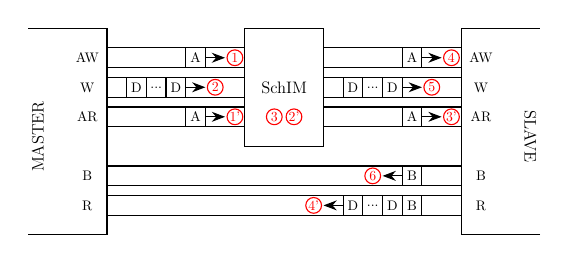
\begin{tikzpicture}[scale=0.5, every node/.style={scale=0.5}]
    % Module Master
    \draw ( 0.0, 0.0) -- ++( 2.0, 0.0) -- ++( 0.0, 5.25) -- ++( -2.0, 0.0);
    \node[rotate=90] at (0.25, 2.5) {\large MASTER};
    % Module Slave
    \draw (13.0, 0.0) -- ++(-2.0, 0.0) -- ++( 0.0, 5.25) -- ++( 2.0, 0.0);
    \node[rotate=270] at (12.75, 2.5) {\large SLAVE};
    % Module SchIM
    \draw ( 5.5, 2.25) rectangle ++( 2.0, 3.00) node [pos=.5] {\large SchIM};
    \draw[red] ( 6.25, 3.0) circle [radius=0.2] node {3};
    \draw[red] ( 6.75, 3.0) circle [radius=0.2] node {2'};
    % AW channel Master to SchIM
    \node at ( 1.5, 4.50) {AW};
    \draw ( 2.0, 4.25) rectangle ++( 3.5, 0.5);
    \draw ( 4.0, 4.25) rectangle ++( 0.5, 0.5)  node[pos=.5] {A};
    \draw[-{Stealth}] ( 4.5, 4.5) -- ++( 0.5, 0.0);
    \draw[red] ( 5.25, 4.5) circle [radius=0.2] node {1};
    \node at ( 11.5, 4.50) {AW};
    % W channel Master to SchIM
    \node at ( 1.5, 3.75) {W};
    \draw ( 2.0, 3.50) rectangle ++( 3.5, 0.5);
    \draw ( 2.5, 3.50) rectangle ++( 0.5, 0.5)  node[pos=.5] {D};
    \draw ( 3.0, 3.50) rectangle ++( 0.5, 0.5)  node[pos=.5] {...};
    \draw ( 3.5, 3.50) rectangle ++( 0.5, 0.5)  node[pos=.5] {D};
    \draw[-{Stealth}] ( 4.0, 3.75) -- ++( 0.5, 0.0);
    \draw[red] ( 4.75, 3.75) circle [radius=0.2] node {2};
    \node at ( 11.5, 3.75) {W};
    % AR channel Master to SchIM
    \node at ( 1.5, 3.00) {AR};
    \draw ( 2.0, 2.75) rectangle ++( 3.5, 0.5);
    \draw ( 4.0, 2.75) rectangle ++( 0.5, 0.5)  node[pos=.5] {A};
    \draw[-{Stealth}] ( 4.5, 3.0) -- ++( 0.5, 0.0);
    \draw[red] ( 5.25, 3.0) circle [radius=0.2] node {1'};
    \node at ( 11.5, 3.0) {AR};
    % AW channel SchIM to Slave
    \draw ( 7.5, 4.25) rectangle ++( 3.5, 0.5);
    \draw ( 9.5, 4.25) rectangle ++( 0.5, 0.5)  node[pos=.5] {A};
    \draw[-{Stealth}] ( 10.0, 4.5) -- ++( 0.5, 0.0);
    \draw[red] (10.75, 4.5) circle [radius=0.2] node {4};
    % W channel SchIM to Slave
    \draw ( 7.5, 3.50) rectangle ++( 3.5, 0.5);
    \draw ( 8.0, 3.50) rectangle ++( 0.5, 0.5)  node[pos=.5] {D};
    \draw ( 8.5, 3.50) rectangle ++( 0.5, 0.5)  node[pos=.5] {...};
    \draw ( 9.0, 3.50) rectangle ++( 0.5, 0.5)  node[pos=.5] {D};
    \draw[-{Stealth}] ( 9.5, 3.75) -- ++( 0.5, 0.0);
    \draw[red] (10.25, 3.75) circle [radius=0.2] node {5};
    % AR channel SchIM to Slave
    \draw ( 7.5, 2.75) rectangle ++( 3.5, 0.5);
    \draw ( 9.5, 2.75) rectangle ++( 0.5, 0.5)  node[pos=.5] {A};
    \draw[-{Stealth}] ( 10.0, 3.0) -- ++( 0.5, 0.0);
    \draw[red] (10.75, 3.0) circle [radius=0.2] node {3'};
    % B channel
    \node at ( 1.5, 1.5) {B};
    \draw ( 2.0, 1.25) rectangle ++( 9.0, 0.5);
    \draw ( 9.5, 1.25) rectangle ++( 0.5, 0.5)  node[pos=.5] {B};
    \draw[-{Stealth}] ( 9.5, 1.5) -- ++(-0.5, 0.0);
    \draw[red] ( 8.75, 1.5) circle [radius=0.2] node {6};
    \node at ( 11.5, 1.50) {B};
    % R channel
    \node at ( 1.5, 0.75) {R};
    \draw ( 2.0, 0.50) rectangle ++( 9.0, 0.5);
    \draw ( 8.0, 0.50) rectangle ++( 0.5, 0.5)  node[pos=.5] {D};
    \draw ( 8.5, 0.50) rectangle ++( 0.5, 0.5)  node[pos=.5] {...};
    \draw ( 9.0, 0.50) rectangle ++( 0.5, 0.5)  node[pos=.5] {D};
    \draw ( 9.5, 0.50) rectangle ++( 0.5, 0.5)  node[pos=.5] {B};
    \draw[-{Stealth}] ( 8.0, 0.75) -- ++(-0.5, 0.0);
    \draw[red] ( 7.25, 0.75) circle [radius=0.2] node {4'};
    \node at ( 11.5, 0.75) {R};
\end{tikzpicture}

            \caption{Caption}
            \label{fig:SchIM_transaction_scheme_figure}
        \end{figure}

    \subsection{Micro-architecture}
        \label{subsec:micro-arch}
        The SchIM module is composed of many sub-modules that can themselves be grouped into three different domains. In fact, as illustrated in figure \ref{fig:MemorEDF_module_schema}, one can distinguish the \emph{scheduling domain}, the \emph{queuing domain} and the \emph{interfacing domain}.

        The scheduling domain encompasses all the sub-modules that enable arbitration of the bus between the transactions issued by the different cores of the PS side. Hence, this domain boasts several transaction schedulers implemented at the hardware level.
        The scheduling policies offered by SchIM include Fixed Priority (FP), Time Division Multiple Access (TDMA), Earliest Deadline First (EDF), Least Laxity First (LLF) and MemGuard (MG).
        Each of the parameters required by the aforementioned algorithms such as the priorities, the periods, the deadlines and the budgets are re-configurable at the run-time thanks to the inclusion of a configuration port.
        Finally, the scheduling domain is also the one in charge of the control of the remaining the SchIM module, driving and selecting the adequate signals and ensuring the coherence and integrity of the data.

        The queuing domain is in charge of the storing the incoming transactions emitted by the PS side.
        The motivation behind the use of queues is implied by the fact that all the masters located on the PS side share a common AXI bus (namely HPM0 as shown in figure \ref{fig:SchIM_overview_schema}).
        Therefore, in order to cancel the Round Robin arbitration policy applied in the PS side and in order to avoid that one high priority core is stalled by a lower priority one, each core is granted a queue within the SchIM module.
        Not only the queues act as containers and buffers for transactions, they also embed logic and provide information to the scheduling domain regarding their current state in order to avoid the queues to overflow or underflow similarly to the producer-consumer problem.
        As suggested by figure \ref{fig:MemorEDF_module_schema}, transactions are inserted to the adequate queues on the basis of the emitters identifier via the dispatcher module.
        Similarly, transactions are evicted from their queue, routed by the selector module and sent directly to the output of the module upon the action of the scheduling domain.

        The interfacing domain encompasses the sub-modules in charge of interfacing both the scheduling domain and the queuing domain with the remaining of the system using the AXI protocol.
        More accurately, three sub-modules compose this domain, the configuration port previously mentioned, the packetizer and the serializer.
        While the packetizer and the serializer serve the purpose of slave and master ports, they are also in charge of respectively transforming the AXI transactions into an equivalent packet and to transform these packets back to a AXI compliant transactions.
        The need for packetizing (i.e. flattening) the AXI transactions is driven by the necessity of storing transactions that are by nature serial within the queuing domain.
        For instance, a standard AXI transaction is composed of one address phase followed by a data phase which itself composed of multiple successive bursts.

        \begin{figure}
            \centering
            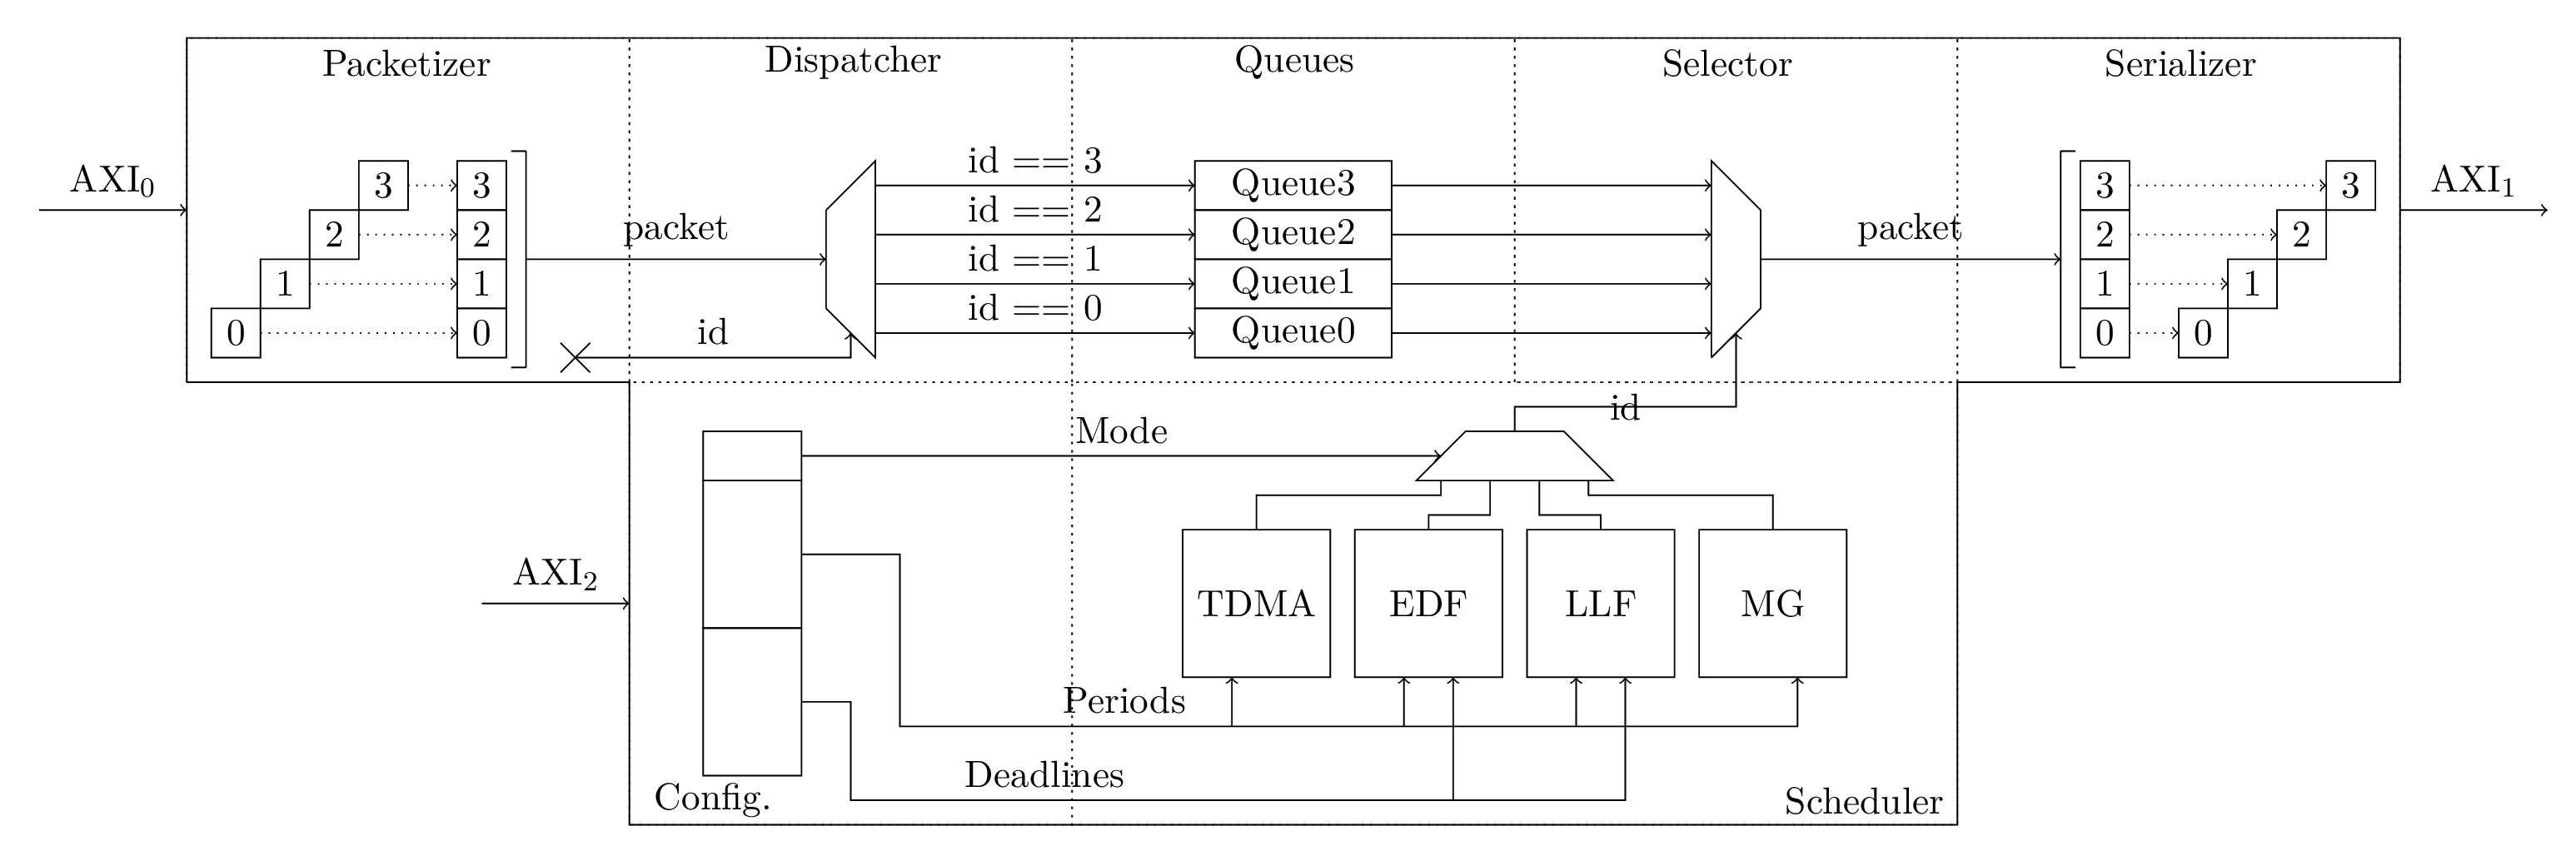
\includegraphics[scale=0.08]{images/MemorEDF_module_schema.png}
            \caption{Caption}
            \label{fig:MemorEDF_module_schema}
        \end{figure}
        
    \subsection{Embedded Schedulers}
        
        \subsubsection{Fixed Priority}
          
        
        \subsubsection{Time Division Multiple Access}
        
        \subsubsection{MemGuard}
          The proposed MemGuard transaction scheduling policy is inspired by the Software-based bus regulation technique ??. The latter has been proved to ensure memory isolation for all the cores involved. Unlike the original MemGuard, the proposed version does not rely on memory budgets and replenishment periods. Instead, it enforces inter-arrival time (i.e. a guaranteed minimal period) between two consecutive transactions emitted by a given core. This distinguishes our approach from \cite{Farshchi2020BRUBR}.
                    
          This scheduling module is implemented as follows. For each of the queues to schedule, the module has a register counting the time elapsed since the start of the period. Once this counter has reached the period set by the user (through the configuration port), the module checks if the queue corresponding to the core contains any transaction. In the case where a transaction is available in the corresponding queue, the latter is forwarded to the output of SchIM (i.e., the serializer) and the counting register is reset to 0. Otherwise, the counting register is blocked to the desired period until a transaction is available for scheduling in the corresponding queue, leading to the counting register to be reset to 0. Any tie between two cores is solved using a fixed priority arbitration defined by the user thanks to the configuration port. 

    \subsection{Transactions Life Cycle}
        \label{subsec:transaction-life-cycle}
        Let us consider a system with four cores (noted $C = \{c_{0}, c_{1}, c_{2}, c_{3}\}$) sending transactions $T = \{t_{0}, t_{1}, ..., t_{n}\}$ to the SchIM module.
        Consequently, the latter boasts four queues (noted $Q = \{q_{0}, q_{1}, q_{2}, q_{3}\}$) buffering the transactions under the form of packets $P = \{p_{0}, p_{1}, ..., p_{n}\}$ where $p_{i} = Packetizer(t_{i})~\forall i \in [0 : n]$.

        In the present example, we will assume $t_{1}$ as being the transaction under analysis.
        The latter is emitted by $c_{2}$ in direction of the SchIM module.
        The packetizer receives this transaction and, once the AXI protocol completed, transform it into an equivalent packet $p_{1} = Packetizer(t_{1})$.
        Following this transformation, the newly created packet is forwarded to the dispatcher which, thanks to the emitter's id embedded within the transaction, is re-routed to the corresponding queue $q_{2}$ (since emitted by $c_{2}$).
        After the insertion of $p_{1}$ in $q_{2}$, the state of the queuing domain is as follows: $q_{0}$ has two packets $p_{0}$ and $p_{k}$ and $q_{2}$ only has $p_{1}$.
        At this point, $q_{0}$ is considered for scheduling by the scheduling domain.
        In consequence, $p_{0}$ is forwarded to the serializer through the selector.
        Simultaneously to the reception of the packet by the serializer, the latter receives an activation signal from the scheduling domain informing the serializer that the packet is valid and that a transaction can be started.
        Similarly to the packetizer, the serializer will transform the packet $p_{0}$ back to its initial AXI transaction form $t_{0} = Serializer(p_{0})$.
        Thereafter, once the $t_{0}$ has been sent, the serializer will inform the scheduling domain via a signal, that he is ready to accept the next packet as input.
        Upon the reception of this signal, the scheduling domain will both re-direct the latter to the queue of the previous packet to indicate that it has been consumed and change the selected queue according to the scheduling policy so that the first packet of this queue can be forwarded to the serializer through the selector module.
        In the present example, the "consumed" signal forwarded by the scheduler is sent to $q_{0}$ which is then empty.
        At this instant, two scenarios are possible:
        \begin{enumerate}
            \item $q_{0}$ is still considered for scheduling following the selected scheduling policy. Therefore, as $q_{0}$ is empty, it outputs an "empty" signal received by the scheduling domain.
                  The latter then decides to not send any activation signal to the serializer because there is nothing left to transmit in the selected queue.
                  In other words, the access to the main memory is being stalled on purpose by the scheduling policy i.e. the scheduling policy is not work conserving.
                  For instance, such a scenario could happen in the case of TDMA or if all the queues are empty.
                  The logic will resume as soon as the selected queue is filled.
            \item $q_{2}$ is now considered instead of $q_{0}$ for scheduling.
                  In this case, the "consumed" signal is repeated to $q_{0}$ while the queue ID changes in order to select $q_{2}$.
                  This results in the packet contained inside $q_{1}$ to be forwarded to the selector.
        \end{enumerate}

\section{PL-to-PS Feedback}
    \todo[inline]{DH: Here, we need to argue why we need a PL feedback (i.e., Queues before the HPM ports), how it can impact SchIM (i.e., nothing can be applied since the queues can be saturated by transaction coming from other cores), how we solved it (i.e., comparators in each queue, comparing the current amount of buffered transactions with a threshold defined by the user through the configuration port, sending an interrupt at the same clock cycle to the PS side, which considers this interrupt line as an FIQ. The FIQ is handled by a routine in the hypervisor that set a DBS instruction (or Data Barrier Synchronisation) in order to kill/stop the core until all the pending transaction have been served.) and how, intuitively, we can choose the values for each proposed Scheduling policies.}
    
    While the combination of the PS and the PL sides offer great opportunities, it also comes with challenges. In fact, each of the HPM ports interfacing the PS and the PL sides (HPM0 and HPM1) have two dedicated queues for read and write transactions. From ??, we know that they all have a depth of 8. Since transactions are being buffered inside SchIm as well as in these port buffers, head-of-the-line blocking can happen. Head-of-the-line blocking can be armful for performance or simply cancel all the efforts put in place to enforce transaction reordering and core isolation. For instance, in the case of a non work-conserving policy (e.g., TDMA), if the HPM port queue gets filled with transaction coming for the same core, 

\section{Evaluation}

The present section aims at evaluating the behavior of the \schim on
the target platform, its overhead and benefits.  First, in subsection
\ref{subsection:considered-architecture}, we review our experimental
setup. Thereafter, we assess the overhead introduced by the \schim in
Section~\ref{subsec:platform-capabilities-and-performance-degradation}.
Section \ref{sec:feedback-pressure} explores the impact of the PL-to-PS feedback
on the control and the performance.
In Section~\ref{subsec:internal-behaviour-of-schim}, an in-depth analysis
of the \schim's behavior is presented. Finally, an evaluation of the
temporal behavior of a set of real-world benchmarks operating through
the \schim is provided in Section~\ref{subsec:isolation}.


\subsection{Experimental Setup}
\label{subsection:considered-architecture}
The \schim has been evaluated using synthetic benchmarks (or
\emph{Memory Bombs}), real benchmarks selected from the San Diego
Vision Benchmark Suite (SD-VBS)~\cite{SD-VBS} and a combination of
the two. Specifically, seven memory-intensive benchmarks have
been selected, i.e. \emph{stitch}, \emph{texture synthesis},
\emph{disparity}, \emph{tracking}, \emph{localization}, \emph{mser}
and \emph{sift}. For our runs, we have considered all the intermediate
input sizes ranging from SQCIF (128$\times$196 pixels) to VGA
(640$\times$480 pixels). When running any benchmark, we use the cache
coloring mechanism implemented in the Jailhouse
hypervisor~\cite{determ_virt} to partition the LLC evenly amongst the
4 cores and to prevent our measurements from being affected by inter-core
cache interference. As a result, each benchmark operates on 1/4 of the
total cache space---256~KB. As extensively discussed
in~\cite{bounding_rtas14, palloc_rtas14}, it is also important to
avoid inter-core DRAM bank conflicts, which can cause the arbitrary
re-ordering of transactions originating from different cores. This is
accomplished by (1) configuring the DRAM controller to disable DRAM
bank interleaving; and (2) by performing static cache
bleaching~\cite{gracioli2019designing, PLIM20} at the \schim's output
to re-compact accesses to colored pages into contiguous DRAM
accesses. In this platform, there are a total of 16 DRAM banks of
256~MB each. Thanks to bleaching, we can assign the full size
of 4 banks (i.e., 1~GB) to each core, instead of being restricted
to only 1/4 of that due to non-overlapping color and bank address
bits.

%  \todo[inline]{RM: this part is a bit redundant with the implementation section. We can remove this section and only keep the description of the routes we are gonna test. See above}
%    The COTS platform used for the following set of experiments, the Xilinx ZCU102 development board, features four cores which, with the LLC, composed the cores cluster. While the \schim can be configured to handle many more masters, in the present set of experiments, only the cores composing this cluster competes for main memory access. Consequently, the \schim module has been configured with four queues (one for each master) as shown in Figure \ref{fig:MemorEDF_module_schema}. Following the discussion in section \ref{sec:pl-to-ps-feedback}, \schim has been configured with two slave ports. Finally, the frequency of the PL side has been pushed to 250~MHz.

%    \todo[inline]{RM: The paragraph below to go into experimental setup}
To evaluate the capabilities of the \schim, two memory routes for
the traffic generated by the cores are compared. The first serves
as baselines, whereas, the last one is the one under analysis and
involves the \schim module.  The first path consists in the cores
directly accessing the main memory. As illustrated in
\fig{fig:PS-PL-diagram}, the traffic simply goes through the
\emph{Main Interconnect} before arriving at the DDR controller. This
path is referred to as the \emph{normal route}.
%In the second path,
%traffic is routed through the PL but without being subject to
%scheduling. In this case, a simple one-to-one connection between one
%of the HPM ports and the HPS port is programmed in the PL. No other
%manipulation on the traversing memory transactions is performed inside
%the PL; we refer to this case as the \emph{simple loop-back}.
%Finally,
Secondly, we consider the case where the \schim module is deployed and in
use to schedule memory traffic generated by the CPUs in the PL. Cores
0 and 1 target HPM1 aperture, while cores 2 and 3 target HPM2. In our
analysis, \schim is used in all the available modes, \replace{i.e., FP, TDMA
, and TS.}{i.e., FP and TDMA.}

\subsection{Platform Capabilities and performance degradation}
\label{subsec:platform-capabilities-and-performance-degradation}
Intuitively and as discussed in~\cite{PLIM20}, redirecting the traffic
coming from the cores to the PL side incurs a performance hit. In
spite of the lower frequency at which the \schim operates (250~MHz),
the theoretical throughput when using both the HPM lanes should be
around 8~GBps. We observe, however, that the achievable throughput
through the HPM ports is a fraction of that due to what appears to be
PS-side internal throttling. For the sake of completeness, we quantify
in \fig{fig:bandwidth_comparison} the maximum bandwidth achieved
through the PL --- and hence through the \schim. Nevertheless, it is
important to remember that the absolute figures are strictly platforms
dependent.

In \fig{fig:bandwidth_comparison}, we have computed the throughput of
one \emph{core under analysis}, here core 0 (noted $C_{0}$) when a
synthetic memory-intensive application is deployed on an increasing
number of cores denoted with the same notation. The first bar cluster
(``Normal'') refers to the throughput measured via the normal
route. The other three clusters capture the observed bandwidth when
traffic is routed through and managed by the \schim.
One cluster is provided for each of the implemented memory scheduling policies,
namely --- from left to right --- \replace{FP, TDMA, and TS}{FP and TDMA}.
As expected, there is a sharp reduction (around 75\%) in terms of absolute
bandwidth. Importantly, however, two aspects need to be
highlighted. First, the bandwidth achieved through the \schim is still
remarkably high and allows studying the behavior of the realistic workload
under custom memory scheduling policies, which is the primary goal of
this research. Second, it emerges that the implemented FP and TDMA
policies are capable of protecting the core under analysis from
inter-core interference, while this is not the case when going through
the normal route
\removed{
, nor when using the TS policy at the \schim.
}


%% for each
%% of the aforementioned paths under all the possible levels of
%% contention. The result of this experiment is display in
%% \fig{fig:bandwidth_comparison}.

%% From , one can observe that in general,
%% the throughput experienced by the core under analysis (i.e., $C_{0}$)
%% is high and that, regardless of the contention level on the normal
%% route, the bandwidth remains high. As mentioned earlier, redirecting
%% the cores' traffic through the PL side has a cost. In fact, in the
%% case with no contention (the left-most bar cluster), the bandwidth
%% experienced by $C_{0}$ when going through the simple loop-back, is
%% reduced by around 75\% compared to the normal route.  Looking at the
%% left-most bar cluster, one can also observe the overhead introduced by
%% having the presence of the \schim on the memory loop-back. The
%% additional drop in bandwidth is approximately 185~MBps.  While the
%% throughput is larger in the case of the \emph{simple loop-back}, it
%% also drops linearly as soon as the contention level increases.  On the
%% other hand, the \schim manages to preserve the same bandwidth, with
%% negligible interference being observed in the most challenging
%% scenario (the right-most bar cluster). In other words, the \schim
%% guarantees performance isolation between the cores with respect to the
%% bus usage.

\begin{figure}
  \centering
%  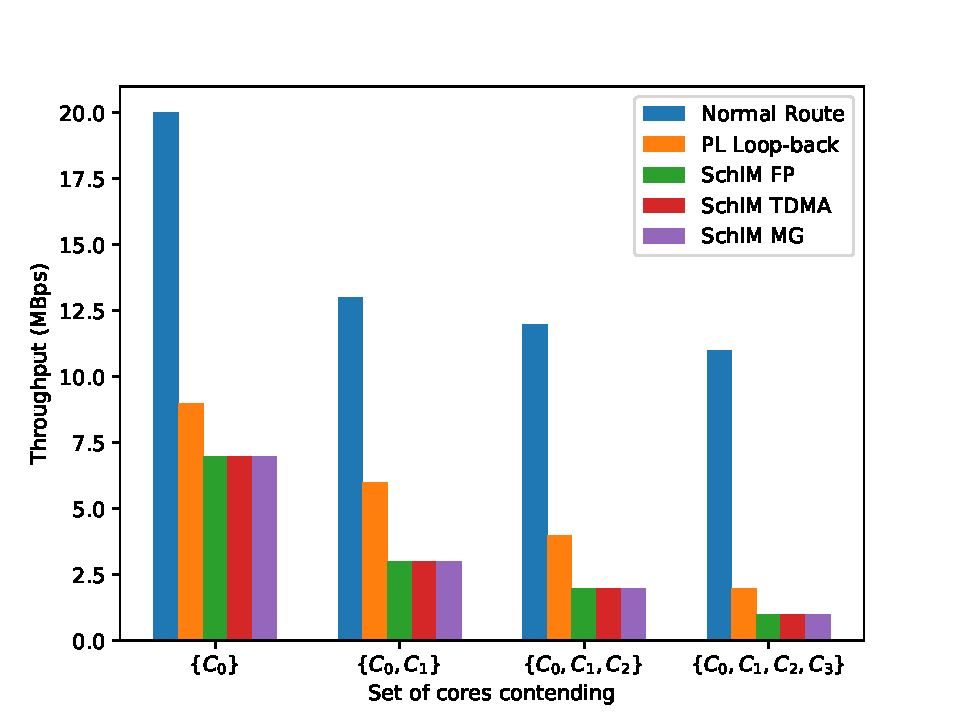
\includegraphics[scale=0.45]{images/bw_comparisons.pdf}
  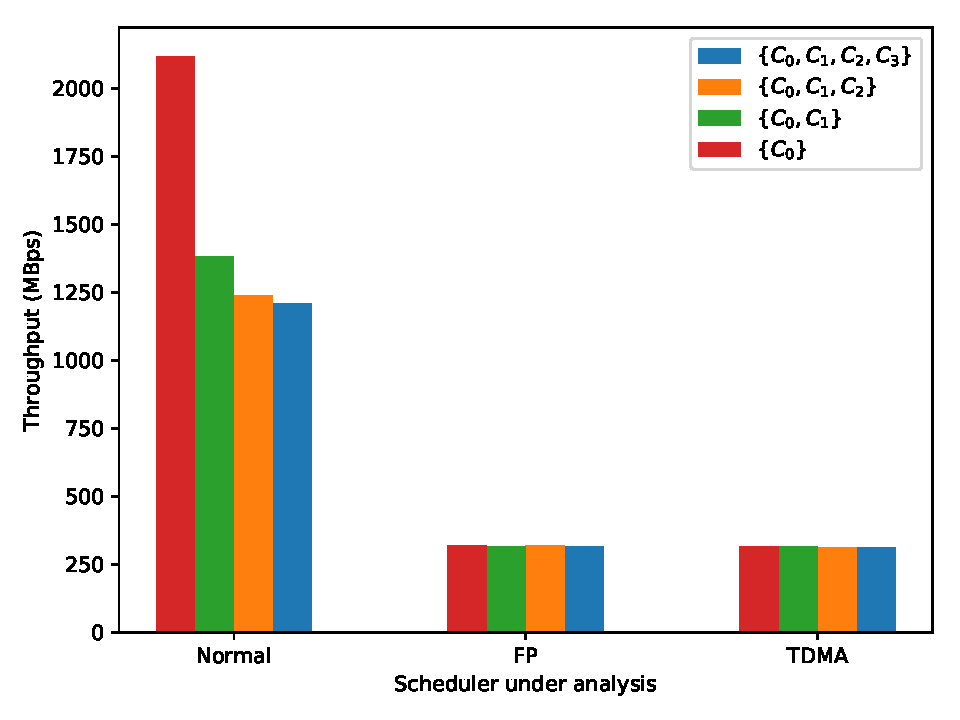
\includegraphics[scale=0.45]{images/bw_comparisons_no_ts.pdf}
  \caption{Bandwidth in MBps for different path under increasing set of cores contending.}
  \label{fig:bandwidth_comparison}
\end{figure}

\subsection{PL-to-PS feedback performance impact}
\label{sec:feedback-pressure}
\begin{figure}[]
  \centering
  \begin{subfigure}{0.9\textwidth}
    \centering
    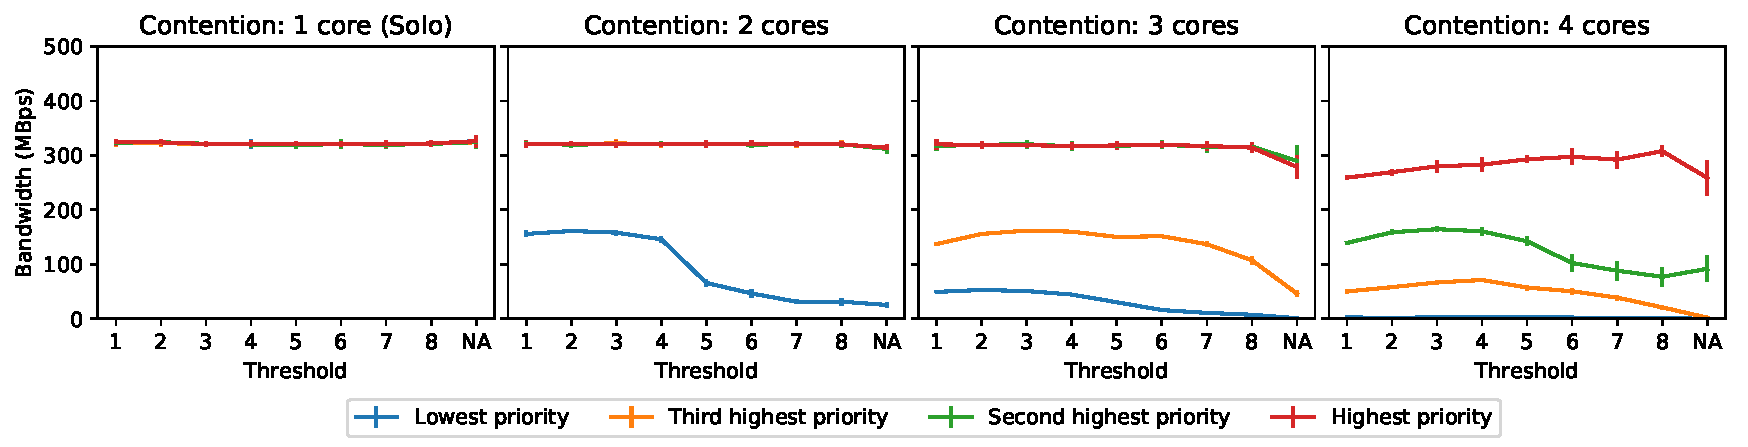
\includegraphics[scale=0.4]{images/fp.pdf}
    \caption{Threshold-Bandwidth relationship curves for the FP scheduler}
    \label{fig:threshold_fp}
  \end{subfigure}
  \hfill
  \begin{subfigure}{0.9\textwidth}
    \centering
    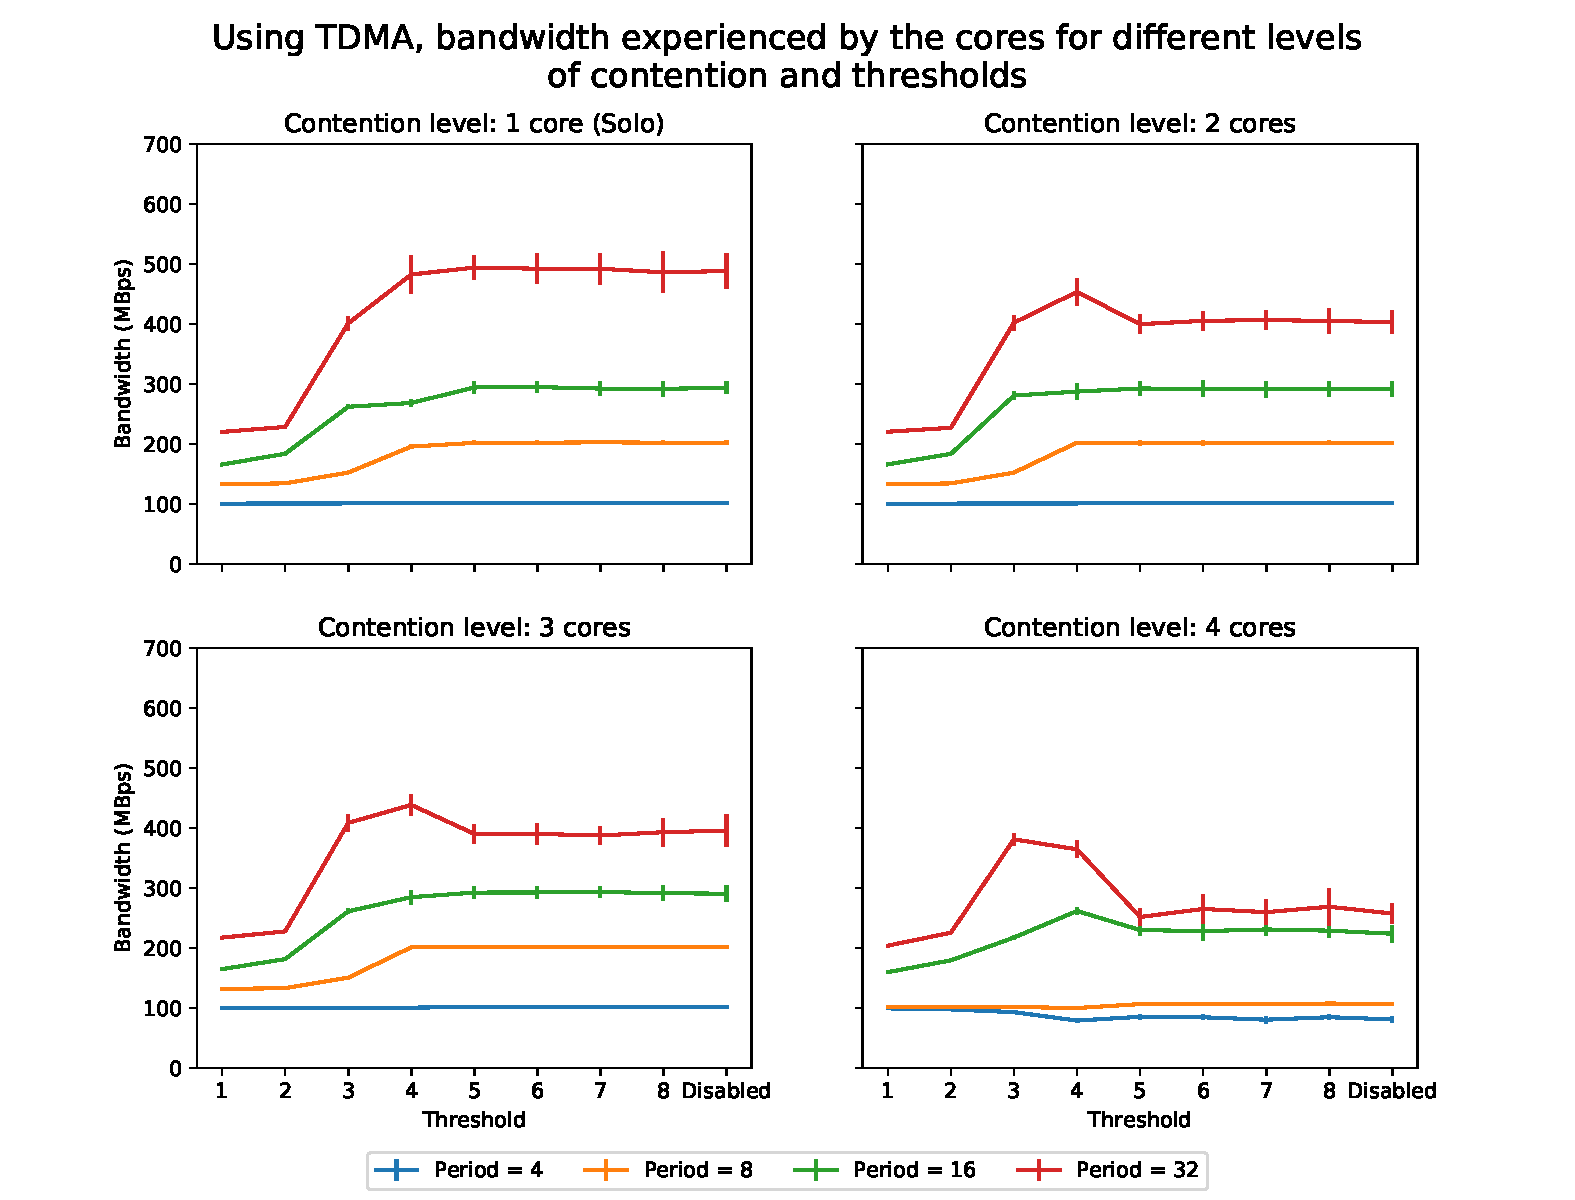
\includegraphics[scale=0.4]{images/tdma.pdf}
    \caption{Threshold-Bandwidth relationship curves for the TDMA scheduler}
    \label{fig:threshold_tdma}
  \end{subfigure}
%  \begin{comment}
%  \hfill
%  \begin{subfigure}{0.9\textwidth}
%    \centering
%    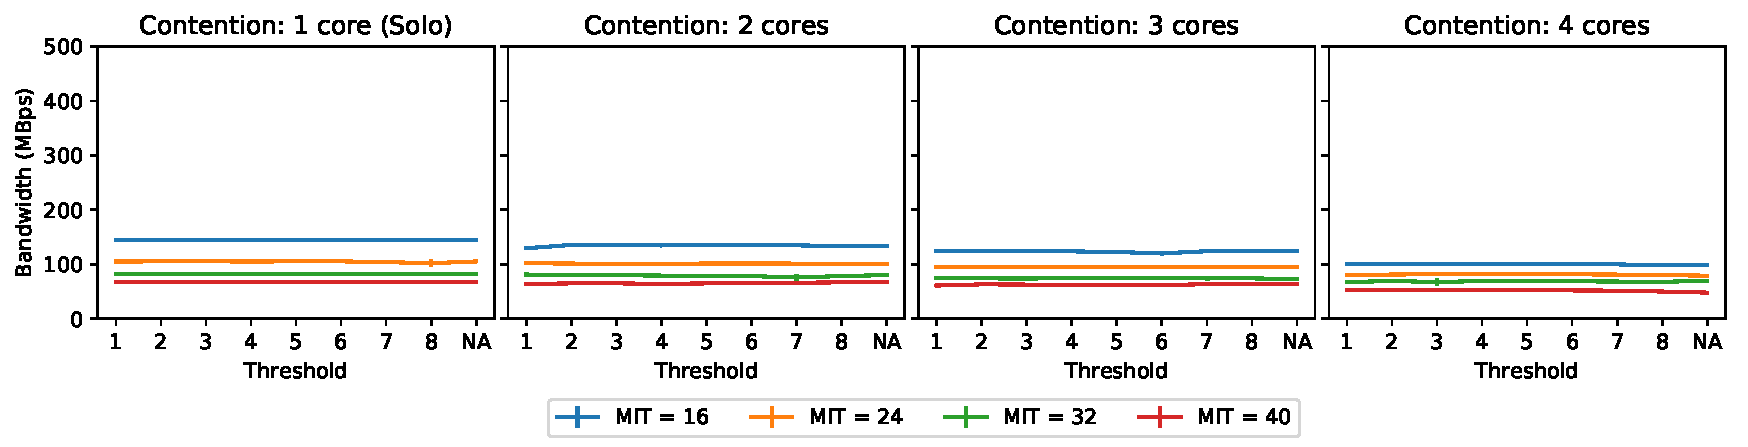
\includegraphics[scale=0.4]{images/ts.pdf}
%    \caption{Threshold-Bandwidth relationship curves for the TS scheduler}
%    \label{fig:threshold_ts}
%  \end{subfigure}
%\end{comment}
\textcolor{red}{TS subfigure removed}
  \caption{Figures showing the impact of the threshold in use on the final bandwidth experinced by the cores for the offered schedulers}
  \label{fig:schim_threshold}
\end{figure}
As mentioned in Section \ref{sec:pl-to-ps-feedback}, the PL-to-PS feedback enables
\schim to regulate the HPM ports buffer occupancy to prevent head-of-line blocking.
Since this feedback directly throttles the desired core, the selection of an adequate
threshold is important to preserve the balance between control and performance.
Therefore, in Figure \ref{fig:schim_threshold}, we have explored the sensitivity
to the threshold for each of the proposed schedulers under different levels of contention.
The thresholds in use range from 1 to 8 and even include the case where the feedback mechanism is disabled
(noted \emph{NA}). The contention is created by up to four co-running cores emitting
write transactions. For each parameter applied to a scheduler (i.e., fixed
priority, TDMA slot or MIT), the co-running cores are assigned the most
demanding parameters available (i.e., the highest priority for FP, the biggest TDMA
slot or the smallest MIT).

In the case of the FP scheduler (Figure \ref{fig:threshold_fp}), one can observe
that when running alone, the threshold has no influence on the throughput.
However, as soon as co-runners are added, the cores start to experience a
decrease in throughput.
Figure \ref{fig:threshold_tdma} shows that the TDMA scheduler is not impacted considerably by the threshold with respect to the throughput. Globally, the
scheduler manages to preserve a constant throughput regardless of the contention
and the assigned slot.
\removed{
Similarly, the TS scheduler is barely impacted by choice of the threshold as
displayed in Figure \ref{fig:threshold_ts}.
}

Nonetheless, under high
contention, one can observe that the throughput of each core is affected.
The fourth inset of Figure \ref{fig:threshold_fp} and \ref{fig:threshold_tdma}
illustrate the importance of the threshold and the PL-to-PL feedback mechanism as a
a considerable drop of throughput can be observed for the highest priority of FP
and for a TDMA period of 32.

Considering these experiments, setting the threshold to four for all the schedulers
seems to bring the best trade-off between control and performance. However, this
value cannot be blindly applied to all cases as this experiment is performed for
a sequential and contiguous access pattern.

\subsection{Internal Behaviour of SchIM}
\label{subsec:internal-behaviour-of-schim}
The next objective is to verify the correct behavior of the schedulers
at the granularity of a clock cycle by observing the inputs,
the outputs and the internal signals and registers of the \schim
module. This is made possible thanks to the \emph{Integrated Logic
  Analyzer} (or ILA) provided by Xilinx \cite{Xilinx-ILA}. The latter
IP can be directly implemented on the PL side, alongside the \schim,
and is able to probe the signals and to store them in a local
memory. For this experiment, a group of relevant internal signals have
been probed and captured during a window of 16384 contiguous clock
cycles. Then, the information has been extracted by post-processing
the data. To characterize the behavior of the three different
policies, the ILA has been instrumented to collect (i) the amount of
transactions being buffered in the queues at each clock cycle
\replace{(inset 1 in \fig{fig:schim_behaviour_fp}, \fig{fig:schim_behaviour_tdma}, and
\fig{fig:schim_behaviour_mg}),}{(inset 1 in \fig{fig:schim_behaviour_fp} and \fig{fig:schim_behaviour_tdma})}
(ii) the rate at which queues receive
new transactions from the cores cluster
\replace{(inset 2 in \fig{fig:schim_behaviour_fp}, \fig{fig:schim_behaviour_tdma}, and
\fig{fig:schim_behaviour_mg}),}{(inset 2 in \fig{fig:schim_behaviour_fp} and \fig{fig:schim_behaviour_tdma})}
 and (iii) the queues ID of each
transaction forwarded by the \schim module
\replace{(inset 3 in \fig{fig:schim_behaviour_fp}, \fig{fig:schim_behaviour_tdma}, and
\fig{fig:schim_behaviour_mg}).}{(inset 3 in \fig{fig:schim_behaviour_fp} and \fig{fig:schim_behaviour_tdma}).}

For the Fixed Priority trace snapshot displayed in
\fig{fig:schim_behaviour_fp}, the following strict priority ordering
has been considered: $C_{0} \succ C_{1} \succ C_{2} \succ C_{3}$ where
the $\succ$ operator means that the left argument has a strictly
higher priority than the right argument. In this experiment, a
regulation threshold of 3 for each core has been used.  As emphasized
by the inset 2 in \fig{fig:schim_behaviour_fp}, the FP scheduler is
able to prioritize the traffic of one core at the expense of the
others according to the priorities assignment. Furthermore, one can
observe that the rate at which the queues receive new transactions
from their associated core is proportional to the priority level in
the priority ordering.  Finally, the third inset in
\fig{fig:schim_behaviour_fp} confirms the correct behavior of the FP
policy.%, with the higher the core's priority, the higher the transaction density at the output of \schim is.
%Thanks to the heat map, one can clearly see that the cores
%with the highest priority also feature the highest density of
%transactions at the output of the \schim.
One can see that the cores with the highest priority also feature the
highest density of transactions at the output of the \schim.

The trace snapshot displayed in \fig{fig:schim_behaviour_tdma} has
been obtained by configuring the \schim module in TDMA mode. For the
sake of clarity, a slot of 256 clock cycles has been set for each
core. Besides, the threshold of each core has been set to 4 to
create sharp transitions.  The insets 2 and 3 of
\fig{fig:schim_behaviour_tdma} clearly show the behavior expected
from a TDMA schedule. In fact, one can clearly see in the latter that
transactions originating from one core are only being repeated out of
the \schim module during a well-defined and periodic time slot of 256 clock cycles. In the inset 2 of \fig{fig:schim_behaviour_tdma}, we can
observe a similar pattern, with transactions arriving only during the
TDMA slot associated with their queue (and indirectly core). Globally,
the rate at which queues receive transactions is steady and constant.
\removed{
The trace snapshot for the TS policy has been obtained with an MIT of
160 clock cycles for each core. Similar to the TDMA experiment, such
period has been set arbitrarily in order to improve the clarity of the
trace snapshot displayed in \fig{fig:schim_behaviour_mg}. Thanks to
the inset 3 in \fig{fig:schim_behaviour_mg}, we can see that under a significant traffic load, the TS mode of the \schim is able to shape
the output traffic. Roughly, the same pattern can be observed in the inset
2 of \fig{fig:schim_behaviour_mg}. However, there is an exception.
In both the second and the third insets, queue 3 (and indirectly core 3)
clearly violates the pattern expected from the TS scheduler. This transaction
leakage is due to a malfunction in the TS scheduler design.
}

%First, one queue can receive more than one transaction. This is due to
%the coarseness of the FIQ feedback regulation. Secondly, some queues
%seem to be prioritized. This can be explained by the fact that in the
%TS scheduler implementation break ties between valid ready transactions
%using a FP policy. In this experiment, since the \schim module is constantly under pressure, there are always ties between the queues and FP is frequently applied.
    \begin{figure}[t]
      \centering
      \begin{subfigure}{0.45\textwidth}
        \centering
        % include first image
        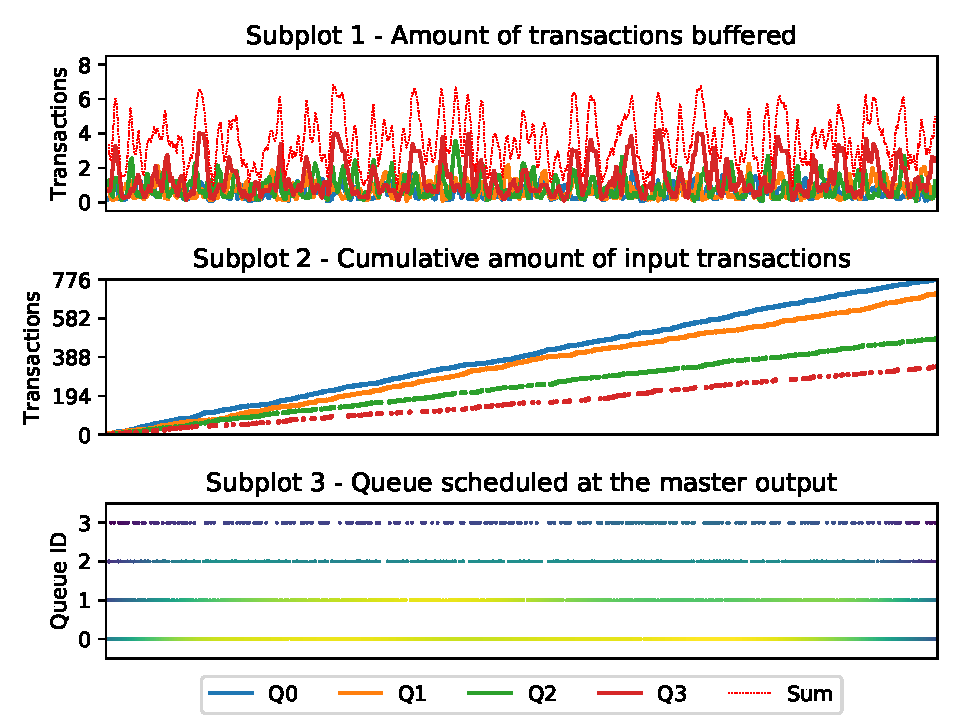
\includegraphics[scale=0.45]{images/SchIM_FP_buffering.pdf}
        \caption{FP with ordering $C_{0} \succ C_{1} \succ C_{2} \succ C_{3}$}
        \label{fig:schim_behaviour_fp}
      \end{subfigure}
      \hfill
      \begin{subfigure}{0.45\textwidth}
        \centering
        % include second image
        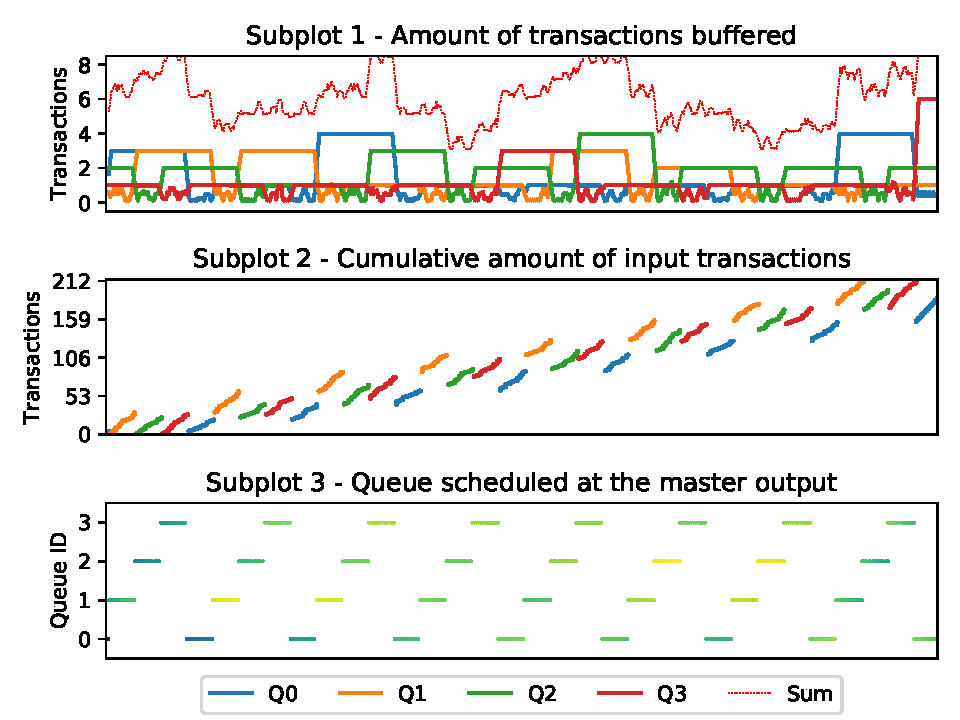
\includegraphics[scale=0.45]{images/SchIM_TDMA_buffering.pdf}
        \caption{TDMA with slots of 256 clock cycles}
        \label{fig:schim_behaviour_tdma}
      \end{subfigure}
      \hfill
      \begin{subfigure}{0.45\textwidth}
  %      \centering
  %      % include second image
  %      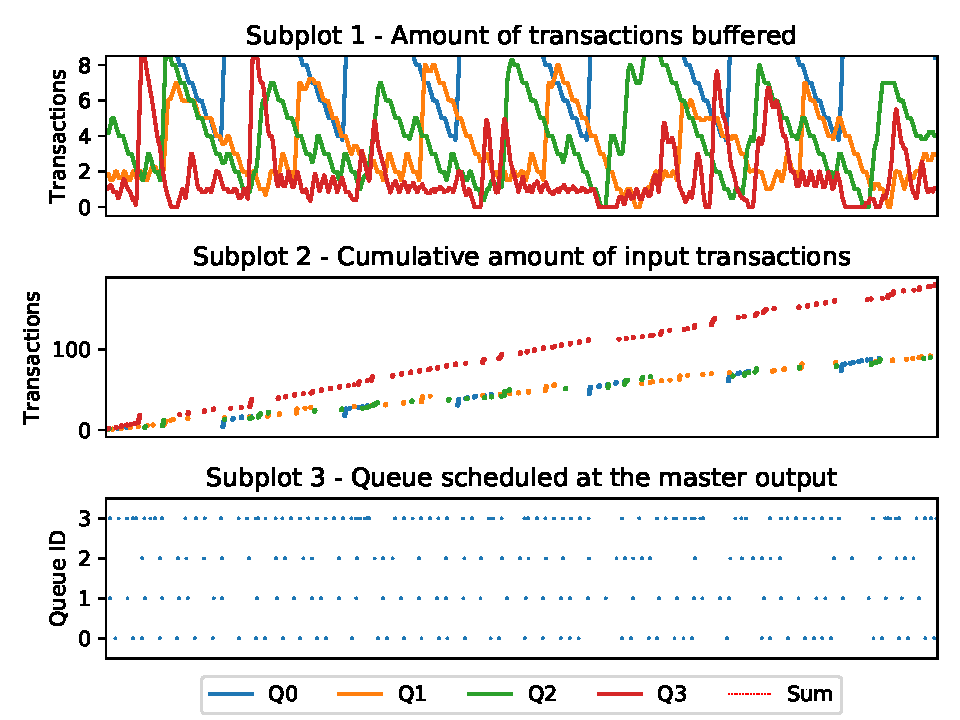
\includegraphics[scale=0.45]{images/SchIM_TS_buffering.pdf}
  %      \caption{TS with min. period of 160 clock cycles}
  %      \label{fig:schim_behaviour_mg}
        \textcolor{red}{TS subfigure removed}
      \end{subfigure}
      \caption{Trace snapshots of SchIM for FP (\ref{fig:schim_behaviour_fp}), TDMA (\ref{fig:schim_behaviour_tdma}) \removed{and TS (\ref{fig:schim_behaviour_mg})}}
      \label{fig:schim_behaviour}
    \end{figure}

\subsection{Memory Isolation}
\label{subsec:isolation}
To evaluate the capability of our \schim with respect to its ability to
ensure performance isolation between the cores, a set of experiments
involving SD-VBS benchmarks were designed. Here, we compare the
execution time of an application on a given core when running alone
(referred to as \emph{Solo}) and when running alongside interfering synthetic
benchmarks (write memory bombs) on all the other cores (referred to as
\emph{Stress}).
For each combination of a route to main memory (i.e., the \emph{normal
route} or the \emph{\schim route}) and scheduler, the result obtained
for \emph{Stress} is normalized with respect to the equivalent configuration
in \emph{Solo}.
%The slowdown compared to the case in which the observed
%benchmark runs alone in the system is computed while taking the same
%route to the main memory (i.e., the \emph{normal route} or the
%\empl{\schim route}).
%It follows that a ratio of 1 denotes the ideal isolation.
The results obtained on the considered benchmarks are listed in
Figure~\ref{fig:isolation_ratio}. All the results in the
Figure~\ref{fig:isolation_ratio} are the aggregation (arithmetic average)
of 30 different runs in the same configuration. Each bar cluster of the Figure~\ref{fig:isolation_ratio} insets represents one of the aforementioned configuration for \emph{Solo} and \emph{Stress}. The height of each bar denotes its normalized execution time.

For this set of experiments, the FP scheduler was configured such that the core under
analysis (i.e., the one running the benchmark) has the highest priority
and a threshold of 8. The other cores are assigned lower priorities and
thresholds matching their priority order (i.e., 4, 2, 1). Under TDMA scheduling, the core under analysis has a slot of 512 clock cycles and a threshold of 14 while the co-runners are assigned slots of 32 and 16 clock cycles with thresholds of 4 and 1.
\removed{
For the TS scheduler, the core under analysis is assigned a MIT of 16 and a threshold of 4, whereas each co-runner has a MIT of 64 and a threshold of 2.
}

The \emph{normal route} is used as a baseline for this experiment
because no scheduling is performed in this configuration.
%The results for
%the simple loop-back are displayed in the left-most column in
%Table~\ref{fig:isolation_ratio}.
The Figure \ref{fig:isolation_ratio} highlights the sensitivity of both
\emph{disparity} and \emph{mser} to inter-core interference on the
\emph{normal route}. This is especially the case for large input sizes
such as \emph{cif} and \emph{vga}. On the other hand, \emph{texture
synthesis} and \emph{localization} do not suffer from inter-core
interference.
Globally, the TDMA scheduler always manages to preserve the isolation of
the core, having execution times under \emph{Stress} similar or smaller than the \emph{normal route}. This is particularly visible for \emph{qcif}, \emph{cif} and \emph{vga} input sizes of \emph{disparity} and \emph{mser}.
%Unlike the \emph{normal route}, the TDMA scheduler manages to mitigate
%the impact of the inter-core interference on the core under analysis for
%\emph{disparity} and \emph{mser}. In fact, for \emph{qcif}, \emph{cif} and
%\emph{vga}, the scheduler is as good or better than the \emph{normal route}.
%In fact, the ratio of all the benchmarks we tested lie in
%the proximity of 1.0, with a maximum inter-core interference of around 7\%.
Similarly, the FP scheduler is also capable of ensuring sound
isolation of the core under analysis.
\removed{
Unfortunately, the TS scheduler generally fails to provide any form of
isolation. This is more than likely due to the logic defect mentioned in
Section \ref{subsec:internal-behaviour-of-schim}. In this case, the transaction leakage
prevents the transaction from the core under analysis to be served as they
unexpectedly occupy the bus, unpredictability delaying the scheduling of the other transactions.
}
% of the core under analysis
%despite having been assigned the highest priority. Even worst, the
%scheduler has a little-to-none impact since its slowdown is comparable
%to that observed on the loop-back path.
%This result can be explained by the fact that despite the enforcement of the FP policy, and its proven correct behavior (see \fig{fig:schim_behaviour_fp}), the
%This
%enforced ordering of transaction is likely overridden by the
%transaction re-ordering mechanisms present in the DDR controller. The
%problem specifically occurs because the access pattern of the
%interfering bombs is sequential, and hence preferably treated by the
%DDR controller. Conversely, the FP scheduler works correctly in
%scenarios like those in \fig{fig:schim_behaviour_fp} because the
%memory access pattern of the core under analysis is sequential as
%well. It follows that the FP policy is mainly useful when performing
%the movement of large, sequential data chunks.
\begin{figure}
    \centering
%    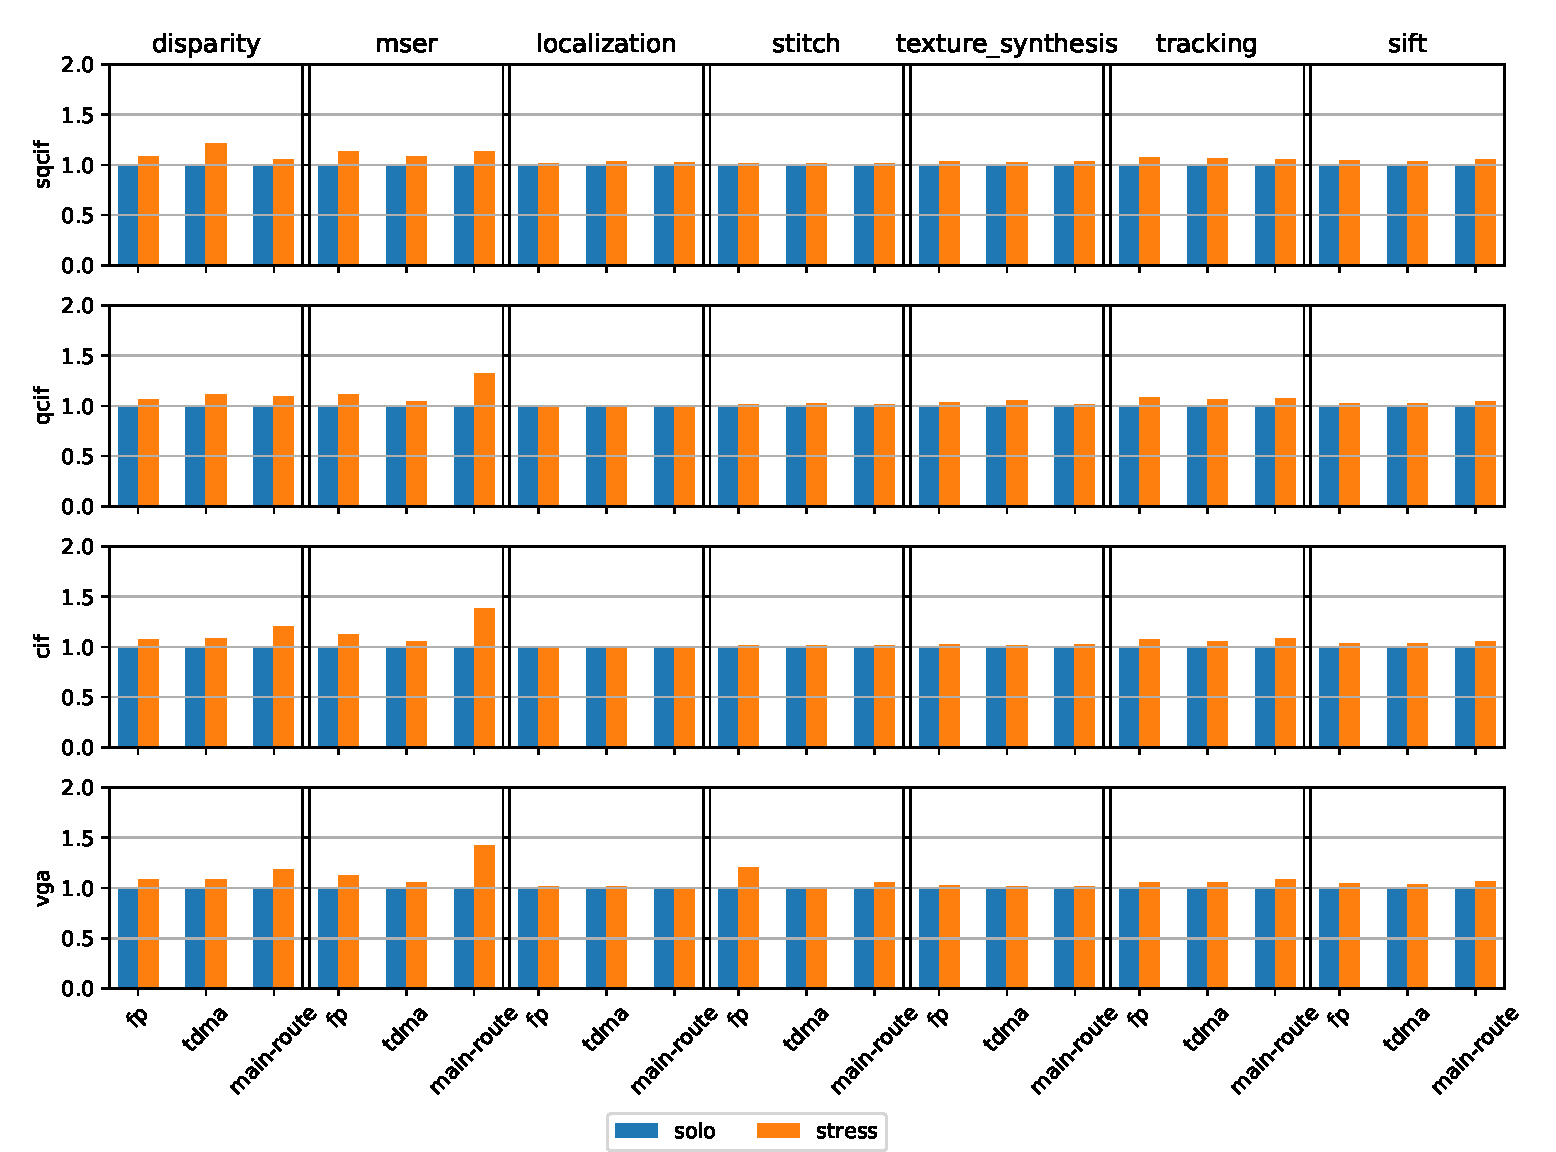
\includegraphics[scale=0.54]{images/Execution_times.pdf}
    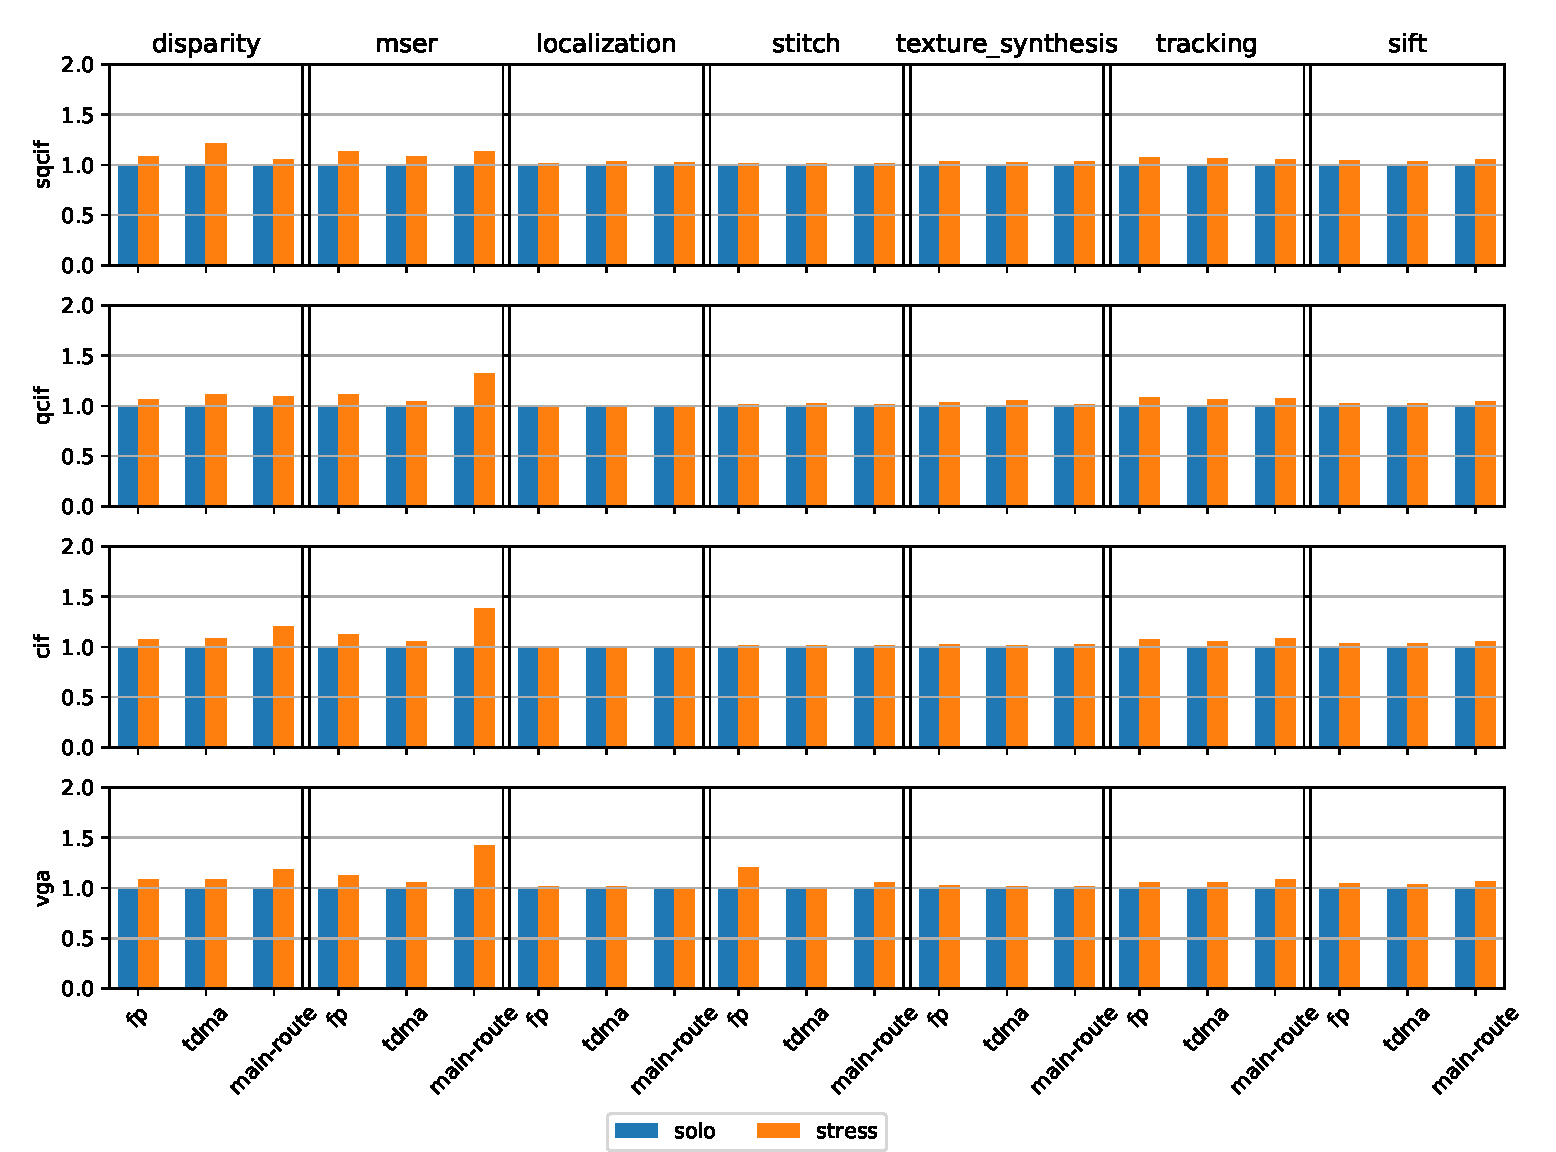
\includegraphics[scale=0.54]{images/Execution_times_no_ts.pdf}
    \caption{Normalized execution time for each benchmark and input size for \emph{Solo} and \emph{Stress}. Each column denotes a given benchmark of the SD-VBS suite, while each row denotes a specific input size (in increasing order from top to bottom).}
    \label{fig:isolation_ratio}
\end{figure}

\section{Discussion \new{and Limitations}}
\label{sec:discussion}
%When comparing the throughput that is experienced by the cores, the normal route always provides a higher throughput in comparison to the the loop-back-based path.
%However, when only comparing those loop-back-based paths, we can see that the price to pay for having \schim is largely compensated by the memory isolation the latter provides.
%In general, redirecting the cores traffic toward the PL side with \schim is interesting in combination with techniques such as  \textit{address bleaching} and \textit{zero-copy recoloring}.
\removed{
Even though the throughput offered by the \emph{normal route} is higher, the
authors argue that comparing the latter's raw performance against \schim is unfair.
Redirecting the CPU-originated memory traffic through the PL side has a cost.
However, this cost is mainly linked to the implementation and the platform capabilities, elements that can be improved by optimization as well as a selection of more aggressive platforms.
The important aspect brought by the proposed framework, \schim, is its capability to individually manipulate memory transactions, opening the door to the study of novel memory scheduling policies.
The PL-to-PS feedback is an interesting regulating mechanism. Moreover, it is entirely transparent to the hypervisor's inmates and uses the fastest route possible to communicate with the PS side. Nonetheless, this feedback mechanism is coarse. Inset 1 of Figure \ref{fig:schim_behaviour_tdma} highlights perfectly this problem. Even though all the queues have been assigned a threshold of 4, the latter is often exceeded. The worst-case being queue 3 exceeding the threshold by 2 on the right side of the plot.
The thresholds used for the FIQ regulation requires to be fine-tuned manually by the user. Future extensions of the \schim will explore the implementation of schedulers capable of dynamically adapting the threshold to maximize the performance and improve the core isolation.
}

\new{ By design, the PLiM module proposed in this paper, the \schim,
  centralizes the memory traffic and its scheduling. A centralized
  design makes sense on the specific target platform because there
  exist only one memory controller and thus a single path between the
  LLC and the DRAM controller. In systems where multiple paths between
  the processing units and the memory controllers exist, for instance
  when multiple controllers and channels are present, a decentralized
  design is to be preferable to better exploit the available memory
  parallelism. In such platforms, a possible avenue could be
  instantiating multiple \schim modules, roughly one per channel, and
  introducing appropriate out-of-band signaling between the modules
  for coordination off the critical path.

  As we mentioned in Section~\ref{subsection:considered-architecture},
  our setup includes the Jailhouse partitioning hypervisor.  While the
  \schim module does not strictly require the PS side to use a
  hypervisor, Jailhouse has been extensively used for the evalution as
  it provides convenient features to control physical memory
  allocation.  For instance, the support for page coloring has been
  used to both partition the LLC space and to easily identify the
  owner of each memory transactions in the \schim (as presented in
  Section~\ref{sec:traffic-accounting}).  However, instead of
  enforcing cache partitioning, one could instead identify the
  ownership of memory transactions by extracting a different subset of
  address bits. For instance, if the physical memory allocated to
  different partitions is not interleaved, then the most significant
  bits of the address can be used to perform traffic accounting. In
  addition, the IPA address virtualization is convenient to
  transparently redirect the memory traffic of the application
  partitions through the PL side, even if they are initially booted
  through the normal route.  Finally, the cores throttling mechanism
  (see Section~\ref{sec:pl-to-ps-feedback}) via the FIQs can be
  implemented at EL3 (Secure Monitor) or in the individual guest OS's
  instead (EL1). Implementing FIQ handling in the hypervisor (EL2),
  however, has the advantage of not requiring any change in the guest
  OS's, as well as not requiring a full switch into secure mode
  compared to an implementation at EL3.

  On the same note, provided that the FIQ lines are not used by the
  inmates, the feedback regulation mechanism is entirely transparent
  to the guest OS's (or even for bare-metal applications) and
  introduces minimum overhead. The Linux kernel do not use FIQs, and
  the same goes for typical RTOS's. Nonetheless, it must be
  acknowledged that defining a FIQ handler to be used for CPU
  throttling might interfere with (and be interfered by) the latency
  of FIQ handling in guest OS's that rely on the same
  functionality. This is mainly because FIQ handling is
  non-preemptive. We also recognize that the PL-to-PS feedback
  mechanism is relatively coarse. Inset 1 of
  Figure~\ref{fig:schim_behaviour_tdma} highlights this problem. Even
  though all the queues have been assigned a threshold of 4, the
  threshold is often exceeded.  The worst-case being queue 3 exceeding
  the threshold by 2 on the right-hand side of the plot. This problem
  can be attributed to the reaction time of the FIQ routine, and to
  the fact that jumping to the FIQ handler itself might cause a few
  memory transactions depending on the cache state. Currently, the
  thresholds used for FIQ-based regulation require to be fine-tuned
  manually by the user. Future extensions of the \schim will explore
  the implementation of schedulers capable of dynamically adapting the
  thresholds to maximize performance and improve isolation. The loss in
  bandwidth caused by routing transactions through the PL
  is important and a serious drawback against the adoption of the
  \schim,}\newbis{compared to the PS-to-DDR4 accesses.}
  \replacebis{The authors impute this drop of bandwidth to the path
  between the PS-side modules on the path from the core cluster to the
  HPM ports rather than on the frequency of the PL side itself. In
  fact, if one assumes a PL frequency of 250MHz and a single-burst
  beat of 128~bits per clock cycle, any bus segment implemented in the
  PL should be able to sustain a throughput of approximately
  3.7GBps. This is in line with the throughput reported
  in~\cite{uiuc-xilinx-port-study}. Moreover, it is important to
  remark that the difference in clock speed between CPUs and PL is
  misleading. This is because transactions originated by the CPUs
  cross a PS-side bus that operates at a much lower
  frequency. Specifically, on our platform the main bus subsystem
  operates at 500MHz whereas the CPUs operate at 1.5GHz. On the other
  hand, while the \schim does introduce some extra latency and thus
  has some impact on the available bandwidth, we can conclude that
  bulk of the penalty arises from the two levels of interconnects
  (CCI+Main Interconnect, see Figure~\ref{fig:PS-PL-diagram}) and
  FIFOs located on the path from the core cluster to the HPM
  ports. Therefore, it constitutes a limitation of the employed
  platform rather than of the proposed design.}{There can be multiple
    reasons for this drop in performance the back-of-the-envelope
    calculation stating that a PL operating at 250MHz should sustain
    a throughput of 3.7GB/s \cite{uiuc-xilinx-port-study}. Secondly,
    our experiments targeted explicitly at this problem have highlighted
    throttling at the HPM ports where bandwidth regulators present
    between HPM ports and the PL\cite{Xilinx-ULTRASCALE-TRM}.
    Finally, transactions originated by the CPUs
    cross a PS-side bus that operates at a much lower
    frequency. Specifically, on our platform, the main bus subsystem
    operates at 500MHz, whereas the CPUs operate at 1.5GHz. On the other
    hand, while the \schim does introduce some extra latency and thus
    has some impact on the available bandwidth, we can conclude that
    the bulk of the penalty arises from the two levels of interconnects
    (CCI+Main Interconnect, see Figure~\ref{fig:PS-PL-diagram}) and
    FIFOs located on the path from the core cluster to the HPM
    ports. Therefore, it constitutes a limitation of the employed
    platform rather than the proposed design.

    By looking at this evidence, the PL itself can sustain much higher
    throughput than what experimentally observed, and that the drop is
    imputable to throttling happening on the PS side. However,
    identifying the real bottleneck in the PS-PL path still requires
    further investigation, such as examining clock-domain crossing and
    HPM-PS QoS regulation, which is a part of our future work.}

\section{Conclusion}
    \begin{itemize}
        \item Such system, under strict conditions cannot quarantee QoS nor Mixed-criticality levels.
        \item In contrast to what has been previously reported, read intensive applications can also become a threat for the system predictability.
    \end{itemize}
    \subsection{Future works}
        \begin{itemize}
            \item Study if the same impact can be found with the attacker targeting a scratch pad memory which frequency could be modify.
            \item Investigate whether this phenomenom can also be observed in other, more recent, ARM core families.
        \end{itemize}


\bibliographystyle{IEEEtranS}
\bibliography{references}

\end{document}
